\documentclass[beamer, xcolor={table,usenames,dvipsnames}]{beamer}
%\usepackage{mathpazo}
\usepackage[T1]{fontenc}
\usepackage[utf8]{inputenc}
\usepackage[ngerman]{babel}
\usepackage[babel,german=quotes]{csquotes}
\usepackage{lmodern} % for removing warning about font shape

%\usetheme{Madrid}
\usetheme{Frankfurt}
%\usetheme{Singapore}
\usecolortheme{crane}

\setbeamertemplate{footline}[frame number] % für Foliennummerierung
\beamertemplatenavigationsymbolsempty % Navigationsleiste 

\AtBeginSection{\frame{\sectionpage}}
\newtranslation[to=ngerman]{Section}{Abschnitt}
\newtranslation[to=ngerman]{Subsection}{Beispielmodell}

\usepackage{etoolbox}
\makeatletter
\patchcmd{\slideentry}{\ifnum#2>0}{\ifnum2>0}{}{\@error{unable to patch}}% replace the subsection number test with a test that always returns true
\makeatother

%\setbeameroption{show notes}

\usepackage{amsmath}
\usepackage{calc}

\usepackage{graphicx} %Zum Einbinden von Grafikdateien
\usepackage[font={footnotesize, sf}]{caption}
\usepackage{subfig}
\graphicspath{{./Abbildungen/}}

\usepackage{booktabs} %Für schönere Tabellen
\usepackage{xspace}

\usepackage{tikz} %Für Skizzen

\usepackage[bibstyle=authortitle, citestyle=authortitle, isbn=false, doi=false,
dashed=false]{biblatex}
\addbibresource{Masterarbeit.bib}
\renewbibmacro*{cite:title}{%
  \printtext[bibhyperref]{%
    \printfield[citetitle]{labeltitle}%
    \setunit{\addcomma\space}%
    \printdate}}

%\usepackage{vmargin} %Fürs Seitenlayout
%\setmarginsrb{2.5cm}{1.5cm}{2cm}{1.5cm}{0mm}{0.5cm}{0mm}{1cm}

%%% Häkchen und Kreuzchen %%%
\usepackage{pifont}% http://ctan.org/pkg/pifont
\newcommand{\cmark}{\ding{51}}%
\newcommand{\xmark}{\ding{55}}%

\usepackage{todonotes}

%%% Eigene Befehle %%%
\newcommand{\was}[1]{\small\textit{#1}}
\newcommand{\noteS}[1]{\todo[color=green!40]{\textbf{Sascha: }#1}}
\newcommand{\noteJ}[1]{\todo[color=blue!40]{\textbf{János: }#1}}
\newcommand{\textfrac}[2]{\hspace{2pt} \frac{\text{#1}}{\text{#2}}}
\newcommand{\eqnref}[1]{\overset{(\ref{#1})}{=}} % Gleichheitszeichen mit Referenz auf die verwendete Gleichung
\newcommand{\defeq}{\vcentcolon=} %Definitions-Gleichheitszeichen
\newcommand{\eqdef}{=\vcentcolon}
\newcommand{\pfrac}[2]{\frac{\partial #1}{\partial #2}}
\newcommand{\markera}[1]{\textcolor{NavyBlue}{#1}} % Farbiger Text 1
\newcommand{\markerb}[1]{\textcolor{Orange}{#1}} % Farbiger Text 2

% Formeln:
\newcommand{\MIPS}[1][]{
  \ifthenelse {\equal {#1} {}}
  {\text{MIPS}} % if argument is blank
  {\text{MIPS}({#1})} % if an optional argument is given
}
\renewcommand{\P}[1]{P_\text{#1}}
\newcommand{\I}[1]{I_\text{#1}}
\newcommand{\itext}[1]{i_\text{#1}}
\newcommand{\T}[1]{T_\text{#1}}
\newcommand{\n}[1]{n_\text{#1}}
\newcommand{\N}[1]{N_\text{#1}}
\renewcommand{\t}[1]{t_\text{#1}}



\title{Ökologische Nachhaltigkeit durch \\ \enquote{Nutzen statt Besitzen}?}
\subtitle{{\small Entwicklung eines Modells zur Ableitung von Kriterien für die Senkung des Umweltverbrauchs durch gemeinschaftliche Produktnutzung}}
\author{Alexander Müller, János Sebestyén}
\date{Universität Osnabrück, 14.07.2015}

\begin{document}

\frame[plain]{\titlepage}


\begin{frame}[plain]
    \begin{center}
        \makebox[\textwidth]{
        \includegraphics<1>[width=\paperwidth]{Luhrmannhof.jpg}
        \includegraphics<2>[width=\paperwidth]{Luhrmannhof50.pdf}
        \includegraphics<3>[width=\paperwidth]{Luhrmannhof50x2.pdf}
        \includegraphics<4>[width=\paperwidth]{Luhrmannhof10x5.pdf}}
    \end{center}
\end{frame}
\frame<beamer>{\tableofcontents}
\section{Einleitung}

\subsection{Thema}
	\begin{frame}{Thema}
        \begin{itemize}
            \item Gemeinschaftliche Nutzung von Produkten \\ Waschsalon,
                Car-Sharing, Werkzeugverleih,\dots
            \item Ökologische Auswirkungen solcher Nutzungsformen im Vergleich
                zur individuellen Nutzung
        \end{itemize}
        	\begin{center}
        		\small
        		\begin{tabular}{p{5cm}p{5cm}}
        			\multicolumn{2}{l}{\textbf{Umwelteffekte durch die
        					Nutzung}}  \\[5pt]
        			\textbf{positiv} & \textbf{negativ} \\
        			\midrule
        			Nutzungsintensivierung  &  Zusätzliche Transporte
        			\\[3pt]
        			Erhöhung der Produktauslastung  & Erhöhung der Produktauslastung \\[3pt]
        			Wartung / Reparaturen &  Wartung / Reparaturen \\[3pt]
        			\bottomrule
        		\end{tabular}
        		\vspace{3pt}

        		Für vollständige Übersicht siehe \cite{scholl_marketing_2009}.
        \end{center}
	\end{frame}



    \subsection{Fragestellung}
	\begin{frame}{Fragestellung}
      \begin{block}{}
	        	\begin{itemize}
	        		\item[] Unter welchen Umständen kann der \textit{Umweltverbrauch} eines Produktes durch gemeinschaftliche Nutzung gegenüber der individuellen Nutzung gesenkt werden?
	        		% \item Was sind die Mechanismen, die den Umweltverbrauch bei gemeinschaftlicher Nutzung bestimmen und wie wirken diese? 
	        		% \item Welche Eigenschaften des Produkts und der Nutzungsform beeinflussen die Wirkung dieser Mechanismen und wie fließen sie ein?
	        	\end{itemize}
      \end{block}
	\end{frame}

    \subsection{Methodik}
	\begin{frame}{Methodik}
            \begin{itemize}
                \pause
                \item Modell-Ansatz: ein Modell je Effekt
                \pause
                \item Produktnutzungssystem
                \begin{itemize}
                    \item Personen 
                    \item Produkte
                    \item Organisation der Nutzung
                \end{itemize}
                \pause
                \item Analyse
                \begin{itemize}
                    \item Übergang von der individuellen zur gemeinschaftlichen Nutzung $\Leftrightarrow$ Veränderung bestimmter Systemparameter
                    \item Umwelteffekt: ein Parameter ändert sich
                    \item Kopplung: mehrere Parameter ändern sich
                \end{itemize}
            \end{itemize}
	\end{frame}

	\begin{frame}{MIPS-Konzept}
		\begin{itemize}
			\item<1-> Operationalisierung des Umweltverbrauchs:
                MIPS\footcite{liedtke_resource_2014}
			\item<2-> MIPS = Materialinput pro Serviceeinheit
			\item<3-> \textbf{Input-Orientierung}: Bilanzierung aller primären Materialbewegungen (Herstellung, Nutzung, Entsorgung) \\
			$\rightarrow$ \emph{Universeller Indikator}
			\item<4-> \textbf{Service-Orientierung}: Bezug auf den erbrachten Nutzen \\
			$\rightarrow$ \emph{Vergleichbarkeit}
		\end{itemize}
		\begin{block}{Grundgleichung}<5->
			$$\text{MIPS} = \frac{I}{S}$$
		\end{block}
	\end{frame}

\section{Modelle}
\subsection{Nutzungsintensivierung}
	\frame{\subsectionpage}
	\begin{frame}{Modellbeschreibung -- Nutzungshäufigkeit}
		\begin{itemize}
			\item<1-> Nutzungsintensivierung = Erhöhung der Nutzungshäufigkeit $h$
            \item<2-> Nutzungsdauer $t$ und Nutzungsmenge $n$ eines Produkts: 
                \\ $n = h \cdot t$
            \item<3-> Nutzungsvorrat $\n{max} \leftrightarrow$ technische
                Lebensdauer $\t{tech}$
            \item<4-> Maximalnutzungsdauer $\t{max}$: $n = \t{max} \cdot h$
            \item<8-> Wir halten fest:
                $$n (h) = \left\{\begin{array}{cl}  h \cdot
                    t_{\text{max}}, & \mbox{falls } h < h^* \\ n_{\text{max}}, &
                    \mbox{sonst} \end{array}\right.$$
			% \item \emph{Gesamt}nutzungsmenge $N$ während $T$: \\ $N = n \cdot P = h \cdot t \cdot P = h \cdot t \cdot p \cdot \frac{T}{t} = h \cdot p \cdot T$
			% \pause
			% \item Mindestproduktanzahl $p_{\text{min}}$: \\ $p \geq p_{\text{min}} \quad  (p, p_{\text{min}} \in \mathbb{N})$
			% \pause
			% \item Servicemenge $S$: \\ $S = S_D = N \cdot A \quad \Leftrightarrow \quad N = \frac{S_D}{A}$ \quad ($A$: Produktauslastung)
			% \pause
			% \item Nutzungshäufigkeit $h$: \\ $h = \frac{N}{p \cdot T} = \frac{S_D}{A \cdot p \cdot T} \qquad h \leq h_\text{max} := \frac{S_D}{A \cdot p_\text{min} \cdot T}$
		\end{itemize}

        % \def\svgscale{0.7}
        \only<1>{\input{./Abbildungen/NI_0.pdf_tex}}
        \only<2>{\input{./Abbildungen/NI_1.pdf_tex}}
        \only<3>{\input{./Abbildungen/NI_2.pdf_tex}}
        \only<4>{\input{./Abbildungen/NI_3.pdf_tex}}
        \only<5>{\input{./Abbildungen/NI_4.pdf_tex}}
        \only<6>{\input{./Abbildungen/NI_5.pdf_tex}}
        \only<7->{\input{./Abbildungen/NI_6.pdf_tex}}
	\end{frame}
    \begin{frame}{Modellbeschreibung -- Service- und Inputs}
        \begin{block}{}
            $$ \MIPS = \frac{I}{S} $$
        \end{block}
        \pause
        \textbf{Serviceeinheiten:}
        \begin{itemize}
            \item konstante Nachfrage $S_D$
            \item diese bezieht sich auf Betrachtungszeitraum $T$
            \item[$\Rightarrow$]  Nutzungseinheiten $N$ (= Serviceeinheiten $S$
                $\cdot$ Auslastung $A$) auch konstant
        \end{itemize}
        \pause
        \textbf{ Inputseite: }
        \begin{itemize}
            \item $I(h) = I_P + \I{fix}$
            \item nutzungsbezogenen Inputs sind konstant
        \end{itemize}
        \pause
        \textbf{Wir erhalten:}
        \begin{block}{}
            $$MIPS = \frac{P(h) \cdot i_P}{S_D} + \frac{\I{fix}}{S_D}$$
        \end{block}

    \end{frame}

	\begin{frame}{Modellbeschreibung -- Produktmenge}
        \visible<1->{\textbf{Was bedeutet die effektive Produktanzahl $P$? }}
		\begin{figure}[h]
			\includegraphics<2>[height=3cm]{Produktanzahlen_1_1}
			\includegraphics<3>[height=3cm]{Produktanzahlen_1_2}
			\includegraphics<4>[height=3cm]{Produktanzahlen_1_3}
			\includegraphics<5->[height=3cm]{Produktanzahlen_2}
		\end{figure}
        \visible<6->{\textbf{Wie bestimmt sich $P$?}}
        \visible<7->{$$\text{Variante 1:} \quad P = p \cdot q = p \cdot
        \frac{T}{t}$$}
        \visible<8->{$$\text{Variante 2:} \quad P (h) = \frac{N}{n(h)} =
        \left\{\begin{array}{cl}  \frac{S_D}{A \cdot h \cdot t_{\text{max}}}, &
            \mbox{falls } h < h^* \\[5pt] \frac{S_D}{A \cdot n_{\text{max}}}, &
            \mbox{sonst} \end{array}\right.$$}
	\end{frame}

	\begin{frame}{Modellbeschreibung -- MIPS-Gleichung}
			$$\text{MIPS}(h) = \frac{I}{S} = \frac{P(h) \cdot i_P + I_{\text{fix}}^h}{S} =
			\frac{I_{\text{fix}}^h}{S_D} + \left\{ \begin{array}{cl}  \frac{i_P}{h \cdot t_{\text{max}} \cdot A}, & \mbox{falls } h < h^* \\[5pt] \frac{i_P}{n_{\text{max}} \cdot A}, & \mbox{sonst} \end{array}\right.$$
		\pause
		\begin{center}
			\resizebox{0.7\linewidth}{!}{
				% Created by tikzDevice version 0.8.1 on 2015-08-28 11:11:44
% !TEX encoding = UTF-8 Unicode
\begin{tikzpicture}[x=1pt,y=1pt]
\definecolor{fillColor}{RGB}{255,255,255}
\path[use as bounding box,fill=fillColor,fill opacity=0.00] (0,0) rectangle (419.17,289.08);
\begin{scope}
\path[clip] ( 46.80, 49.20) rectangle (417.97,221.88);
\definecolor{drawColor}{RGB}{190,190,190}

\path[draw=drawColor,line width= 0.4pt,line join=round,line cap=round] (404.22,108.89) --
	(381.63,108.89) --
	(361.83,108.89) --
	(344.33,108.89) --
	(328.75,108.89) --
	(314.79,108.89) --
	(302.21,108.89) --
	(290.82,108.89) --
	(280.45,108.89) --
	(270.98,108.89) --
	(262.29,108.89) --
	(254.29,108.89) --
	(246.90,108.89) --
	(240.05,108.89) --
	(233.69,108.89) --
	(227.76,108.89) --
	(222.23,108.89) --
	(217.05,108.89) --
	(212.19,108.89) --
	(207.62,108.89) --
	(203.33,108.89) --
	(199.27,108.89) --
	(195.44,108.89) --
	(191.82,108.89) --
	(188.38,108.89) --
	(185.12,108.89) --
	(182.02,108.89) --
	(179.08,108.89) --
	(176.27,108.89) --
	(173.59,109.25) --
	(171.03,109.87) --
	(168.59,110.50) --
	(166.25,111.12) --
	(164.01,111.75) --
	(161.87,112.37) --
	(159.81,113.00) --
	(157.83,113.62) --
	(155.93,114.25) --
	(154.10,114.87) --
	(152.35,115.50) --
	(150.65,116.12) --
	(149.02,116.75) --
	(147.45,117.37) --
	(145.93,118.00) --
	(144.46,118.62) --
	(143.04,119.25) --
	(141.67,119.87) --
	(140.35,120.50) --
	(139.07,121.12) --
	(137.82,121.75) --
	(136.62,122.37) --
	(135.45,123.00) --
	(134.32,123.62) --
	(133.23,124.25) --
	(132.16,124.87) --
	(131.13,125.50) --
	(130.12,126.12) --
	(129.14,126.75) --
	(128.19,127.37) --
	(127.27,128.00) --
	(126.37,128.62) --
	(125.50,129.25) --
	(124.64,129.87) --
	(123.81,130.50) --
	(123.00,131.12) --
	(122.22,131.75) --
	(121.45,132.37) --
	(120.70,133.00) --
	(119.97,133.62) --
	(119.25,134.25) --
	(118.55,134.87) --
	(117.87,135.50) --
	(117.21,136.12) --
	(116.56,136.75) --
	(115.92,137.37) --
	(115.30,138.00) --
	(114.70,138.62) --
	(114.10,139.24) --
	(113.52,139.87) --
	(112.95,140.49) --
	(112.40,141.12) --
	(111.85,141.74) --
	(111.32,142.37) --
	(110.80,142.99) --
	(110.29,143.62) --
	(109.78,144.24) --
	(109.29,144.87) --
	(108.81,145.49) --
	(108.34,146.12) --
	(107.88,146.74) --
	(107.42,147.37) --
	(106.98,147.99) --
	(106.54,148.62) --
	(106.11,149.24) --
	(105.69,149.87) --
	(105.28,150.49) --
	(104.87,151.12) --
	(104.47,151.74) --
	(104.08,152.37) --
	(103.70,152.99) --
	(103.32,153.62) --
	(102.95,154.24) --
	(102.58,154.87) --
	(102.22,155.49) --
	(101.87,156.12) --
	(101.52,156.74) --
	(101.18,157.37) --
	(100.85,157.99) --
	(100.52,158.62) --
	(100.19,159.24) --
	( 99.87,159.87) --
	( 99.56,160.49) --
	( 99.25,161.12) --
	( 98.95,161.74) --
	( 98.65,162.37) --
	( 98.35,162.99) --
	( 98.06,163.62) --
	( 97.78,164.24) --
	( 97.49,164.87) --
	( 97.22,165.49) --
	( 96.94,166.12) --
	( 96.68,166.74) --
	( 96.41,167.37) --
	( 96.15,167.99) --
	( 95.89,168.62) --
	( 95.64,169.24) --
	( 95.39,169.87) --
	( 95.14,170.49) --
	( 94.90,171.12) --
	( 94.66,171.74) --
	( 94.42,172.37) --
	( 94.19,172.99) --
	( 93.96,173.62) --
	( 93.73,174.24) --
	( 93.51,174.86) --
	( 93.29,175.49) --
	( 93.07,176.11) --
	( 92.85,176.74) --
	( 92.64,177.36) --
	( 92.43,177.99) --
	( 92.22,178.61) --
	( 92.02,179.24) --
	( 91.82,179.86) --
	( 91.62,180.49) --
	( 91.42,181.11) --
	( 91.23,181.74) --
	( 91.04,182.36) --
	( 90.85,182.99) --
	( 90.66,183.61) --
	( 90.48,184.24) --
	( 90.29,184.86) --
	( 90.11,185.49) --
	( 89.94,186.11) --
	( 89.76,186.74) --
	( 89.59,187.36) --
	( 89.42,187.99) --
	( 89.25,188.61) --
	( 89.08,189.24) --
	( 88.91,189.86) --
	( 88.75,190.49) --
	( 88.59,191.11) --
	( 88.43,191.74) --
	( 88.27,192.36) --
	( 88.11,192.99) --
	( 87.96,193.61) --
	( 87.81,194.24) --
	( 87.65,194.86) --
	( 87.50,195.49) --
	( 87.36,196.11) --
	( 87.21,196.74) --
	( 87.07,197.36) --
	( 86.92,197.99) --
	( 86.78,198.61) --
	( 86.64,199.24) --
	( 86.50,199.86) --
	( 86.36,200.49) --
	( 86.23,201.11) --
	( 86.09,201.74) --
	( 85.96,202.36) --
	( 85.83,202.99) --
	( 85.70,203.61) --
	( 85.57,204.24) --
	( 85.44,204.86) --
	( 85.32,205.49) --
	( 85.19,206.11) --
	( 85.07,206.74) --
	( 84.95,207.36) --
	( 84.82,207.99) --
	( 84.70,208.61) --
	( 84.59,209.24) --
	( 84.47,209.86) --
	( 84.35,210.49) --
	( 84.24,211.11) --
	( 84.12,211.73) --
	( 84.01,212.36) --
	( 83.90,212.98) --
	( 83.79,213.61) --
	( 83.68,214.23) --
	( 83.57,214.86) --
	( 83.46,215.48);
\definecolor{drawColor}{RGB}{0,0,0}
\definecolor{fillColor}{RGB}{255,255,255}

\path[draw=drawColor,line width= 0.4pt,line join=round,line cap=round,fill=fillColor] (402.23,106.90) rectangle (406.21,110.89);

\path[draw=drawColor,line width= 0.4pt,line join=round,line cap=round,fill=fillColor] (230.39,106.90) rectangle (234.38,110.89);

\path[draw=drawColor,line width= 0.4pt,line join=round,line cap=round,fill=fillColor] (173.11,106.90) rectangle (177.10,110.89);

\path[draw=drawColor,line width= 0.4pt,line join=round,line cap=round,fill=fillColor] (144.47,115.78) rectangle (148.46,119.77);

\path[draw=drawColor,line width= 0.4pt,line join=round,line cap=round,fill=fillColor] (127.29,124.66) rectangle (131.28,128.65);

\path[draw=drawColor,line width= 0.4pt,line join=round,line cap=round,fill=fillColor] (115.83,133.55) rectangle (119.82,137.53);

\path[draw=drawColor,line width= 0.4pt,line join=round,line cap=round,fill=fillColor] (107.65,142.43) rectangle (111.64,146.42);

\path[draw=drawColor,line width= 0.4pt,line join=round,line cap=round,fill=fillColor] (101.51,151.31) rectangle (105.50,155.30);

\path[draw=drawColor,line width= 0.4pt,line join=round,line cap=round,fill=fillColor] ( 96.74,160.19) rectangle (100.73,164.18);

\path[draw=drawColor,line width= 0.4pt,line join=round,line cap=round,fill=fillColor] ( 92.92,169.08) rectangle ( 96.91,173.06);

\path[draw=drawColor,line width= 0.4pt,line join=round,line cap=round,fill=fillColor] ( 89.80,177.96) rectangle ( 93.78,181.95);

\path[draw=drawColor,line width= 0.4pt,line join=round,line cap=round,fill=fillColor] ( 87.19,186.84) rectangle ( 91.18,190.83);

\path[draw=drawColor,line width= 0.4pt,line join=round,line cap=round,fill=fillColor] ( 84.99,195.73) rectangle ( 88.98,199.71);

\path[draw=drawColor,line width= 0.4pt,line join=round,line cap=round,fill=fillColor] ( 83.10,204.61) rectangle ( 87.09,208.60);

\path[draw=drawColor,line width= 0.4pt,line join=round,line cap=round,fill=fillColor] ( 81.46,213.49) rectangle ( 85.45,217.48);
\end{scope}
\begin{scope}
\path[clip] (  0.00,  0.00) rectangle (419.17,289.08);
\definecolor{drawColor}{RGB}{0,0,0}

\node[text=drawColor,anchor=base,inner sep=0pt, outer sep=0pt, scale=  1.00] at (232.38,  3.60) {Nutzungsh"aufigkeit $h$ [NE/Jahr]};

\node[text=drawColor,rotate= 90.00,anchor=base,inner sep=0pt, outer sep=0pt, scale=  1.00] at (  8.40,135.54) {MIPS [kg/SE]};
\end{scope}
\begin{scope}
\path[clip] ( 46.80, 49.20) rectangle (417.97,221.88);
\definecolor{drawColor}{RGB}{0,0,0}

\path[draw=drawColor,line width= 0.4pt,dash pattern=on 1pt off 3pt ,line join=round,line cap=round] (175.10, 49.20) -- (175.10,221.88);
\end{scope}
\begin{scope}
\path[clip] (  0.00,  0.00) rectangle (419.17,289.08);
\definecolor{drawColor}{RGB}{0,0,0}

\node[text=drawColor,anchor=base,inner sep=0pt, outer sep=0pt, scale=  1.20] at (232.38,275.88) {\bfseries Materialintensit"at pro Service-Einheit MIPS$(h)$};
\end{scope}
\begin{scope}
\path[clip] (  0.00,  0.00) rectangle (419.17,289.08);
\definecolor{drawColor}{RGB}{0,0,0}

\path[draw=drawColor,line width= 0.4pt,line join=round,line cap=round] ( 60.55, 49.20) -- (404.22, 49.20);

\path[draw=drawColor,line width= 0.4pt,line join=round,line cap=round] ( 60.55, 49.20) -- ( 60.55, 43.20);

\path[draw=drawColor,line width= 0.4pt,line join=round,line cap=round] (129.28, 49.20) -- (129.28, 43.20);

\path[draw=drawColor,line width= 0.4pt,line join=round,line cap=round] (175.10, 49.20) -- (175.10, 43.20);

\path[draw=drawColor,line width= 0.4pt,line join=round,line cap=round] (198.02, 49.20) -- (198.02, 43.20);

\path[draw=drawColor,line width= 0.4pt,line join=round,line cap=round] (266.75, 49.20) -- (266.75, 43.20);

\path[draw=drawColor,line width= 0.4pt,line join=round,line cap=round] (335.48, 49.20) -- (335.48, 43.20);

\path[draw=drawColor,line width= 0.4pt,line join=round,line cap=round] (404.22, 49.20) -- (404.22, 43.20);

\node[text=drawColor,anchor=base,inner sep=0pt, outer sep=0pt, scale=  1.00] at ( 60.55, 27.60) {0};

\node[text=drawColor,anchor=base,inner sep=0pt, outer sep=0pt, scale=  1.00] at (129.28, 27.60) {200};

\node[text=drawColor,anchor=base,inner sep=0pt, outer sep=0pt, scale=  1.00] at (175.10, 27.60) {$h^*$};

\node[text=drawColor,anchor=base,inner sep=0pt, outer sep=0pt, scale=  1.00] at (198.02, 27.60) {400};

\node[text=drawColor,anchor=base,inner sep=0pt, outer sep=0pt, scale=  1.00] at (266.75, 27.60) {600};

\node[text=drawColor,anchor=base,inner sep=0pt, outer sep=0pt, scale=  1.00] at (335.48, 27.60) {800};

\node[text=drawColor,anchor=base,inner sep=0pt, outer sep=0pt, scale=  1.00] at (404.22, 27.60) {1000};

\path[draw=drawColor,line width= 0.4pt,line join=round,line cap=round] ( 46.80, 55.60) -- ( 46.80,215.48);

\path[draw=drawColor,line width= 0.4pt,line join=round,line cap=round] ( 46.80, 55.60) -- ( 40.80, 55.60);

\path[draw=drawColor,line width= 0.4pt,line join=round,line cap=round] ( 46.80, 82.24) -- ( 40.80, 82.24);

\path[draw=drawColor,line width= 0.4pt,line join=round,line cap=round] ( 46.80,108.89) -- ( 40.80,108.89);

\path[draw=drawColor,line width= 0.4pt,line join=round,line cap=round] ( 46.80,108.89) -- ( 40.80,108.89);

\path[draw=drawColor,line width= 0.4pt,line join=round,line cap=round] ( 46.80,108.89) -- ( 40.80,108.89);

\path[draw=drawColor,line width= 0.4pt,line join=round,line cap=round] ( 46.80,117.77) -- ( 40.80,117.77);

\path[draw=drawColor,line width= 0.4pt,line join=round,line cap=round] ( 46.80,126.66) -- ( 40.80,126.66);

\path[draw=drawColor,line width= 0.4pt,line join=round,line cap=round] ( 46.80,135.54) -- ( 40.80,135.54);

\path[draw=drawColor,line width= 0.4pt,line join=round,line cap=round] ( 46.80,144.42) -- ( 40.80,144.42);

\path[draw=drawColor,line width= 0.4pt,line join=round,line cap=round] ( 46.80,153.31) -- ( 40.80,153.31);

\path[draw=drawColor,line width= 0.4pt,line join=round,line cap=round] ( 46.80,162.19) -- ( 40.80,162.19);

\path[draw=drawColor,line width= 0.4pt,line join=round,line cap=round] ( 46.80,171.07) -- ( 40.80,171.07);

\path[draw=drawColor,line width= 0.4pt,line join=round,line cap=round] ( 46.80,179.95) -- ( 40.80,179.95);

\path[draw=drawColor,line width= 0.4pt,line join=round,line cap=round] ( 46.80,188.84) -- ( 40.80,188.84);

\path[draw=drawColor,line width= 0.4pt,line join=round,line cap=round] ( 46.80,197.72) -- ( 40.80,197.72);

\path[draw=drawColor,line width= 0.4pt,line join=round,line cap=round] ( 46.80,206.60) -- ( 40.80,206.60);

\path[draw=drawColor,line width= 0.4pt,line join=round,line cap=round] ( 46.80,215.48) -- ( 40.80,215.48);

\node[text=drawColor,rotate= 90.00,anchor=base,inner sep=0pt, outer sep=0pt, scale=  1.00] at ( 32.40, 55.60) {0};

\node[text=drawColor,rotate= 90.00,anchor=base,inner sep=0pt, outer sep=0pt, scale=  1.00] at ( 32.40, 82.24) {1};

\node[text=drawColor,rotate= 90.00,anchor=base,inner sep=0pt, outer sep=0pt, scale=  1.00] at ( 32.40,108.89) {2};

\node[text=drawColor,rotate= 90.00,anchor=base,inner sep=0pt, outer sep=0pt, scale=  1.00] at ( 32.40,135.54) {3};

\node[text=drawColor,rotate= 90.00,anchor=base,inner sep=0pt, outer sep=0pt, scale=  1.00] at ( 32.40,162.19) {4};

\node[text=drawColor,rotate= 90.00,anchor=base,inner sep=0pt, outer sep=0pt, scale=  1.00] at ( 32.40,188.84) {5};

\node[text=drawColor,rotate= 90.00,anchor=base,inner sep=0pt, outer sep=0pt, scale=  1.00] at ( 32.40,215.48) {6};

\path[draw=drawColor,line width= 0.4pt,line join=round,line cap=round] ( 83.46,221.88) -- (404.22,221.88);

\path[draw=drawColor,line width= 0.4pt,line join=round,line cap=round] ( 83.46,221.88) -- ( 83.46,227.88);

\path[draw=drawColor,line width= 0.4pt,line join=round,line cap=round] ( 85.09,221.88) -- ( 85.09,227.88);

\path[draw=drawColor,line width= 0.4pt,line join=round,line cap=round] ( 86.98,221.88) -- ( 86.98,227.88);

\path[draw=drawColor,line width= 0.4pt,line join=round,line cap=round] ( 89.19,221.88) -- ( 89.19,227.88);

\path[draw=drawColor,line width= 0.4pt,line join=round,line cap=round] ( 91.79,221.88) -- ( 91.79,227.88);

\path[draw=drawColor,line width= 0.4pt,line join=round,line cap=round] ( 94.91,221.88) -- ( 94.91,227.88);

\path[draw=drawColor,line width= 0.4pt,line join=round,line cap=round] ( 98.73,221.88) -- ( 98.73,227.88);

\path[draw=drawColor,line width= 0.4pt,line join=round,line cap=round] (103.51,221.88) -- (103.51,227.88);

\path[draw=drawColor,line width= 0.4pt,line join=round,line cap=round] (109.64,221.88) -- (109.64,227.88);

\path[draw=drawColor,line width= 0.4pt,line join=round,line cap=round] (117.83,221.88) -- (117.83,227.88);

\path[draw=drawColor,line width= 0.4pt,line join=round,line cap=round] (129.28,221.88) -- (129.28,227.88);

\path[draw=drawColor,line width= 0.4pt,line join=round,line cap=round] (146.46,221.88) -- (146.46,227.88);

\path[draw=drawColor,line width= 0.4pt,line join=round,line cap=round] (175.10,221.88) -- (175.10,227.88);

\path[draw=drawColor,line width= 0.4pt,line join=round,line cap=round] (232.38,221.88) -- (232.38,227.88);

\path[draw=drawColor,line width= 0.4pt,line join=round,line cap=round] (404.22,221.88) -- (404.22,227.88);

\node[text=drawColor,anchor=base,inner sep=0pt, outer sep=0pt, scale=  1.00] at ( 83.46,236.28) {15};

\node[text=drawColor,anchor=base,inner sep=0pt, outer sep=0pt, scale=  1.00] at (103.51,236.28) {8};

\node[text=drawColor,anchor=base,inner sep=0pt, outer sep=0pt, scale=  1.00] at (117.83,236.28) {6};

\node[text=drawColor,anchor=base,inner sep=0pt, outer sep=0pt, scale=  1.00] at (146.46,236.28) {4};

\node[text=drawColor,anchor=base,inner sep=0pt, outer sep=0pt, scale=  1.00] at (175.10,236.28) {3};

\node[text=drawColor,anchor=base,inner sep=0pt, outer sep=0pt, scale=  1.00] at (232.38,236.28) {2};

\node[text=drawColor,anchor=base,inner sep=0pt, outer sep=0pt, scale=  1.00] at (404.22,236.28) {1};

\path[draw=drawColor,line width= 0.4pt,line join=round,line cap=round] ( 46.80, 49.20) --
	(417.97, 49.20) --
	(417.97,221.88) --
	( 46.80,221.88) --
	( 46.80, 49.20);

\node[text=drawColor,anchor=base,inner sep=0pt, outer sep=0pt, scale=  1.00] at (232.38,254.28) {parallele Produktanzahl $p$};
\end{scope}
\end{tikzpicture}

			}
		\end{center}
	\end{frame}

	\begin{frame}{Ergebnis des Modells zur Nutzungsintensivierung}		
        \begin{block}{}
            Senkung des Umweltverbrauchs durch Nutzungsintensivierung genau dann
            möglich, wenn $ h < h^*$ gilt, der Nutzungsvorrat des Produkts also
            nicht aufgebraucht wird.
        \end{block}
	\end{frame}

    \subsection{Modellkopplung: Nutzungsintensivierung und zusätzliche Transporte}
    \frame{\subsectionpage}

    \begin{frame}{Konzeption}
    	\begin{itemize}
    		\item<1-> Grundproblem: \\ Nutzungsintensivierung $\Leftrightarrow$ zusätzliche Transporte
    		\item<2-> Tradeoff:
	    		\begin{itemize}
	    			\item Nutzungsintensivierung: MIPS $\searrow$ oder $\rightarrow$
	    			\item Zusätzliche Transporte: MIPS $\nearrow$ oder $\rightarrow$
	    		\end{itemize}
    		\item<3-> Frage: Wann ist die Gesamtwirkung positiv? \\[1em]
    		% \item<4-> Zusammenhang: \emph{Größe} des gemeinschaftlichen Systems
	    	% 	\begin{itemize}
	    	% 		\item Je größer das System, desto mehr Produkte werden eingespart.
	    	% 		\item Je größer das System, desto mehr zusätzliche Transporte.
	    	% 	\end{itemize}
    	\end{itemize}
    \end{frame}
    \begin{frame}{Beschreibung des Szenarios}
        \begin{minipage}[t]{0.55\textwidth}
            \vspace{0pt}
            \only<1>{
\includegraphics[height=0.65\textheight]{Kopplung_2_Geometrie_1}}
            \only<2>{\includegraphics[height=0.65\textheight]{Kopplung_2_Geometrie_2}}
            \only<3>{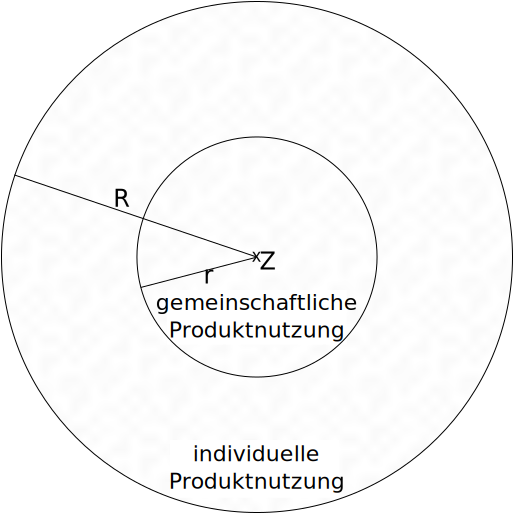
\includegraphics[height=0.65\textheight]{Kopplung_2_Geometrie_3}}
            \only<4>{\includegraphics[height=0.65\textheight]{Kopplung_2_Geometrie_4}}
            \only<5>{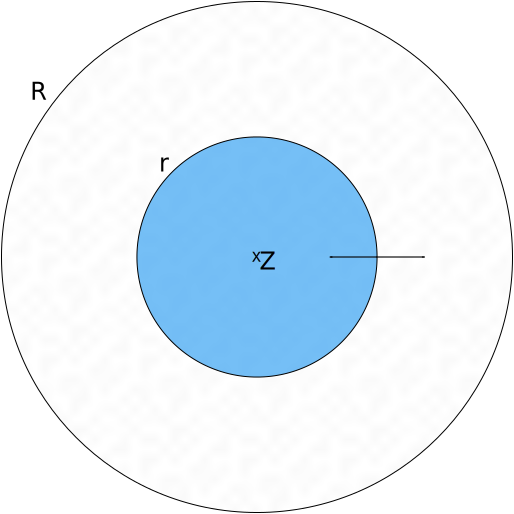
\includegraphics[height=0.65\textheight]{Kopplung_2_Geometrie_5}}
        \end{minipage}
        \begin{minipage}[t]{0.43\textwidth}
            \vspace{0pt} 
            \only<1>{}
            \only<2>{Homogen verteilte Personen-Standorte}
            \only<3>{
                Zwei Teilnutzungssysteme:
                \begin{itemize}
                    \item gemeinschaftliches Nutzungssystem mit $h^\text{gem}$
                    \item individuelles Nutzungssystem mit $h^\text{ind}$
                \end{itemize}
                
                Es gilt:
                $$h^\text{gem} > h^\text{gem} $$
            }
            \only<4>{
                \begin{itemize}
                \item Individuelles Nutzungssystem: keine Transporte\\
                    $\Rightarrow d^\text{ind} = 0$
                \item Gemeinschaftliches Nutzungssystem: Transporte zwischen
                    Zentrum $Z$ und Personen-Standorten\\
                    $\Rightarrow d^\text{gem} = \frac{2}{3}r$
                \end{itemize}
            }
            \only<5>{
                Variation: \emph{Radius} des gemeinschaftlichen Nutzungssystems
                \begin{itemize}
                    \item Je größer das System, desto mehr Produkte
                        werden eingespart.
                    \item Je größer das System, desto mehr
                        zusätzliche Transporte.
                \end{itemize}
            }
        \end{minipage}
    \end{frame}


    \begin{frame}{Modellbeschreibung}
        \begin{itemize}
            \pause
            \item MIPS-Gleichung:\\
                $\text{MIPS}(r) = \frac{I_P + I_\Theta + I_\text{fix}^{h,d}}{S_D}$
			\pause
            \item Transportbezogene Material-Inputs:\\
                $I_\Theta \propto S_D^\text{gem} \cdot d^\text{gem} \propto r^2 \cdot r
                = r^3$
			\pause
            \item Produktbezogene Material-Inputs:\\
                $ I_P \propto P \propto r^2 \cdot \left(
                \frac{q^\text{gem}}{h^\text{gem}} - \frac{q^\text{ind}}{h^\text{ind}}
                \right) + c_1 \qquad (c_1 \dots \text{Konstante})$
        \end{itemize}
        \pause
        \begin{block}{Modell: Nutzungsintensivierung und zusätzliche Transporte}
             $$\text{MIPS}(r) = c_2 \cdot r^2 \cdot \left( \frac{q^\text{gem}}{h^\text{gem}} - \frac{q^\text{ind}}{h^\text{ind}} \right) + c_3 \cdot r^3 + c_4$$
        \end{block}
    \end{frame}

    \begin{frame}{Modellanalyse}
       	\begin{block}{Modell: Nutzungsintensivierung und zusätzliche Transporte}<1->
       		$$\text{MIPS}(r) = c_2 \cdot r^2 \cdot \left( \frac{q^\text{gem}}{h^\text{gem}} - \frac{q^\text{ind}}{h^\text{ind}} \right) + c_3 \cdot r^3 + c_4$$
       	\end{block}
    	\only<1-2>{% Created by tikzDevice version 0.8.1 on 2015-07-12 20:46:16
% !TEX encoding = UTF-8 Unicode
\begin{tikzpicture}[x=1pt,y=1pt]
\definecolor{fillColor}{RGB}{255,255,255}
\path[use as bounding box,fill=fillColor,fill opacity=0.00] (0,0) rectangle (317.99,115.63);
\begin{scope}
\path[clip] ( 14.40, 27.00) rectangle (149.99, 97.63);
\definecolor{drawColor}{RGB}{0,0,0}

\path[draw=drawColor,line width= 0.4pt,line join=round,line cap=round] ( 19.42, 51.42) --
	( 19.55, 51.42) --
	( 19.67, 51.42) --
	( 19.80, 51.42) --
	( 19.92, 51.42) --
	( 20.05, 51.42) --
	( 20.18, 51.42) --
	( 20.30, 51.42) --
	( 20.43, 51.42) --
	( 20.55, 51.42) --
	( 20.68, 51.42) --
	( 20.80, 51.42) --
	( 20.93, 51.42) --
	( 21.06, 51.42) --
	( 21.18, 51.42) --
	( 21.31, 51.42) --
	( 21.43, 51.42) --
	( 21.56, 51.42) --
	( 21.68, 51.42) --
	( 21.81, 51.42) --
	( 21.94, 51.42) --
	( 22.06, 51.42) --
	( 22.19, 51.42) --
	( 22.31, 51.42) --
	( 22.44, 51.42) --
	( 22.56, 51.42) --
	( 22.69, 51.42) --
	( 22.82, 51.42) --
	( 22.94, 51.42) --
	( 23.07, 51.42) --
	( 23.19, 51.42) --
	( 23.32, 51.42) --
	( 23.44, 51.42) --
	( 23.57, 51.42) --
	( 23.69, 51.42) --
	( 23.82, 51.42) --
	( 23.95, 51.42) --
	( 24.07, 51.42) --
	( 24.20, 51.42) --
	( 24.32, 51.42) --
	( 24.45, 51.42) --
	( 24.57, 51.42) --
	( 24.70, 51.42) --
	( 24.83, 51.42) --
	( 24.95, 51.42) --
	( 25.08, 51.42) --
	( 25.20, 51.42) --
	( 25.33, 51.42) --
	( 25.45, 51.42) --
	( 25.58, 51.42) --
	( 25.71, 51.42) --
	( 25.83, 51.42) --
	( 25.96, 51.42) --
	( 26.08, 51.42) --
	( 26.21, 51.42) --
	( 26.33, 51.42) --
	( 26.46, 51.42) --
	( 26.59, 51.42) --
	( 26.71, 51.42) --
	( 26.84, 51.42) --
	( 26.96, 51.43) --
	( 27.09, 51.43) --
	( 27.21, 51.43) --
	( 27.34, 51.43) --
	( 27.47, 51.43) --
	( 27.59, 51.43) --
	( 27.72, 51.43) --
	( 27.84, 51.43) --
	( 27.97, 51.43) --
	( 28.09, 51.43) --
	( 28.22, 51.43) --
	( 28.34, 51.43) --
	( 28.47, 51.43) --
	( 28.60, 51.43) --
	( 28.72, 51.43) --
	( 28.85, 51.43) --
	( 28.97, 51.44) --
	( 29.10, 51.44) --
	( 29.22, 51.44) --
	( 29.35, 51.44) --
	( 29.48, 51.44) --
	( 29.60, 51.44) --
	( 29.73, 51.44) --
	( 29.85, 51.44) --
	( 29.98, 51.44) --
	( 30.10, 51.44) --
	( 30.23, 51.44) --
	( 30.36, 51.44) --
	( 30.48, 51.45) --
	( 30.61, 51.45) --
	( 30.73, 51.45) --
	( 30.86, 51.45) --
	( 30.98, 51.45) --
	( 31.11, 51.45) --
	( 31.24, 51.45) --
	( 31.36, 51.45) --
	( 31.49, 51.45) --
	( 31.61, 51.46) --
	( 31.74, 51.46) --
	( 31.86, 51.46) --
	( 31.99, 51.46) --
	( 32.12, 51.46) --
	( 32.24, 51.46) --
	( 32.37, 51.46) --
	( 32.49, 51.47) --
	( 32.62, 51.47) --
	( 32.74, 51.47) --
	( 32.87, 51.47) --
	( 32.99, 51.47) --
	( 33.12, 51.47) --
	( 33.25, 51.47) --
	( 33.37, 51.48) --
	( 33.50, 51.48) --
	( 33.62, 51.48) --
	( 33.75, 51.48) --
	( 33.87, 51.48) --
	( 34.00, 51.48) --
	( 34.13, 51.49) --
	( 34.25, 51.49) --
	( 34.38, 51.49) --
	( 34.50, 51.49) --
	( 34.63, 51.49) --
	( 34.75, 51.50) --
	( 34.88, 51.50) --
	( 35.01, 51.50) --
	( 35.13, 51.50) --
	( 35.26, 51.50) --
	( 35.38, 51.51) --
	( 35.51, 51.51) --
	( 35.63, 51.51) --
	( 35.76, 51.51) --
	( 35.89, 51.51) --
	( 36.01, 51.52) --
	( 36.14, 51.52) --
	( 36.26, 51.52) --
	( 36.39, 51.52) --
	( 36.51, 51.53) --
	( 36.64, 51.53) --
	( 36.77, 51.53) --
	( 36.89, 51.53) --
	( 37.02, 51.54) --
	( 37.14, 51.54) --
	( 37.27, 51.54) --
	( 37.39, 51.54) --
	( 37.52, 51.55) --
	( 37.64, 51.55) --
	( 37.77, 51.55) --
	( 37.90, 51.55) --
	( 38.02, 51.56) --
	( 38.15, 51.56) --
	( 38.27, 51.56) --
	( 38.40, 51.57) --
	( 38.52, 51.57) --
	( 38.65, 51.57) --
	( 38.78, 51.58) --
	( 38.90, 51.58) --
	( 39.03, 51.58) --
	( 39.15, 51.59) --
	( 39.28, 51.59) --
	( 39.40, 51.59) --
	( 39.53, 51.60) --
	( 39.66, 51.60) --
	( 39.78, 51.60) --
	( 39.91, 51.61) --
	( 40.03, 51.61) --
	( 40.16, 51.61) --
	( 40.28, 51.62) --
	( 40.41, 51.62) --
	( 40.54, 51.62) --
	( 40.66, 51.63) --
	( 40.79, 51.63) --
	( 40.91, 51.63) --
	( 41.04, 51.64) --
	( 41.16, 51.64) --
	( 41.29, 51.65) --
	( 41.42, 51.65) --
	( 41.54, 51.65) --
	( 41.67, 51.66) --
	( 41.79, 51.66) --
	( 41.92, 51.67) --
	( 42.04, 51.67) --
	( 42.17, 51.68) --
	( 42.29, 51.68) --
	( 42.42, 51.68) --
	( 42.55, 51.69) --
	( 42.67, 51.69) --
	( 42.80, 51.70) --
	( 42.92, 51.70) --
	( 43.05, 51.71) --
	( 43.17, 51.71) --
	( 43.30, 51.72) --
	( 43.43, 51.72) --
	( 43.55, 51.73) --
	( 43.68, 51.73) --
	( 43.80, 51.74) --
	( 43.93, 51.74) --
	( 44.05, 51.75) --
	( 44.18, 51.75) --
	( 44.31, 51.76) --
	( 44.43, 51.76) --
	( 44.56, 51.77) --
	( 44.68, 51.77) --
	( 44.81, 51.78) --
	( 44.93, 51.78) --
	( 45.06, 51.79) --
	( 45.19, 51.79) --
	( 45.31, 51.80) --
	( 45.44, 51.80) --
	( 45.56, 51.81) --
	( 45.69, 51.82) --
	( 45.81, 51.82) --
	( 45.94, 51.83) --
	( 46.07, 51.83) --
	( 46.19, 51.84) --
	( 46.32, 51.84) --
	( 46.44, 51.85) --
	( 46.57, 51.86) --
	( 46.69, 51.86) --
	( 46.82, 51.87) --
	( 46.94, 51.88) --
	( 47.07, 51.88) --
	( 47.20, 51.89) --
	( 47.32, 51.89) --
	( 47.45, 51.90) --
	( 47.57, 51.91) --
	( 47.70, 51.91) --
	( 47.82, 51.92) --
	( 47.95, 51.93) --
	( 48.08, 51.93) --
	( 48.20, 51.94) --
	( 48.33, 51.95) --
	( 48.45, 51.96) --
	( 48.58, 51.96) --
	( 48.70, 51.97) --
	( 48.83, 51.98) --
	( 48.96, 51.98) --
	( 49.08, 51.99) --
	( 49.21, 52.00) --
	( 49.33, 52.01) --
	( 49.46, 52.01) --
	( 49.58, 52.02) --
	( 49.71, 52.03) --
	( 49.84, 52.04) --
	( 49.96, 52.04) --
	( 50.09, 52.05) --
	( 50.21, 52.06) --
	( 50.34, 52.07) --
	( 50.46, 52.07) --
	( 50.59, 52.08) --
	( 50.72, 52.09) --
	( 50.84, 52.10) --
	( 50.97, 52.11) --
	( 51.09, 52.12) --
	( 51.22, 52.12) --
	( 51.34, 52.13) --
	( 51.47, 52.14) --
	( 51.59, 52.15) --
	( 51.72, 52.16) --
	( 51.85, 52.17) --
	( 51.97, 52.18) --
	( 52.10, 52.18) --
	( 52.22, 52.19) --
	( 52.35, 52.20) --
	( 52.47, 52.21) --
	( 52.60, 52.22) --
	( 52.73, 52.23) --
	( 52.85, 52.24) --
	( 52.98, 52.25) --
	( 53.10, 52.26) --
	( 53.23, 52.27) --
	( 53.35, 52.28) --
	( 53.48, 52.29) --
	( 53.61, 52.30) --
	( 53.73, 52.31) --
	( 53.86, 52.32) --
	( 53.98, 52.33) --
	( 54.11, 52.34) --
	( 54.23, 52.35) --
	( 54.36, 52.36) --
	( 54.49, 52.37) --
	( 54.61, 52.38) --
	( 54.74, 52.39) --
	( 54.86, 52.40) --
	( 54.99, 52.41) --
	( 55.11, 52.42) --
	( 55.24, 52.43) --
	( 55.37, 52.44) --
	( 55.49, 52.45) --
	( 55.62, 52.46) --
	( 55.74, 52.47) --
	( 55.87, 52.48) --
	( 55.99, 52.49) --
	( 56.12, 52.50) --
	( 56.24, 52.52) --
	( 56.37, 52.53) --
	( 56.50, 52.54) --
	( 56.62, 52.55) --
	( 56.75, 52.56) --
	( 56.87, 52.57) --
	( 57.00, 52.58) --
	( 57.12, 52.60) --
	( 57.25, 52.61) --
	( 57.38, 52.62) --
	( 57.50, 52.63) --
	( 57.63, 52.64) --
	( 57.75, 52.66) --
	( 57.88, 52.67) --
	( 58.00, 52.68) --
	( 58.13, 52.69) --
	( 58.26, 52.71) --
	( 58.38, 52.72) --
	( 58.51, 52.73) --
	( 58.63, 52.74) --
	( 58.76, 52.76) --
	( 58.88, 52.77) --
	( 59.01, 52.78) --
	( 59.14, 52.80) --
	( 59.26, 52.81) --
	( 59.39, 52.82) --
	( 59.51, 52.84) --
	( 59.64, 52.85) --
	( 59.76, 52.86) --
	( 59.89, 52.88) --
	( 60.02, 52.89) --
	( 60.14, 52.90) --
	( 60.27, 52.92) --
	( 60.39, 52.93) --
	( 60.52, 52.95) --
	( 60.64, 52.96) --
	( 60.77, 52.97) --
	( 60.89, 52.99) --
	( 61.02, 53.00) --
	( 61.15, 53.02) --
	( 61.27, 53.03) --
	( 61.40, 53.05) --
	( 61.52, 53.06) --
	( 61.65, 53.07) --
	( 61.77, 53.09) --
	( 61.90, 53.10) --
	( 62.03, 53.12) --
	( 62.15, 53.13) --
	( 62.28, 53.15) --
	( 62.40, 53.17) --
	( 62.53, 53.18) --
	( 62.65, 53.20) --
	( 62.78, 53.21) --
	( 62.91, 53.23) --
	( 63.03, 53.24) --
	( 63.16, 53.26) --
	( 63.28, 53.27) --
	( 63.41, 53.29) --
	( 63.53, 53.31) --
	( 63.66, 53.32) --
	( 63.79, 53.34) --
	( 63.91, 53.36) --
	( 64.04, 53.37) --
	( 64.16, 53.39) --
	( 64.29, 53.41) --
	( 64.41, 53.42) --
	( 64.54, 53.44) --
	( 64.67, 53.46) --
	( 64.79, 53.47) --
	( 64.92, 53.49) --
	( 65.04, 53.51) --
	( 65.17, 53.53) --
	( 65.29, 53.54) --
	( 65.42, 53.56) --
	( 65.54, 53.58) --
	( 65.67, 53.60) --
	( 65.80, 53.61) --
	( 65.92, 53.63) --
	( 66.05, 53.65) --
	( 66.17, 53.67) --
	( 66.30, 53.69) --
	( 66.42, 53.70) --
	( 66.55, 53.72) --
	( 66.68, 53.74) --
	( 66.80, 53.76) --
	( 66.93, 53.78) --
	( 67.05, 53.80) --
	( 67.18, 53.82) --
	( 67.30, 53.83) --
	( 67.43, 53.85) --
	( 67.56, 53.87) --
	( 67.68, 53.89) --
	( 67.81, 53.91) --
	( 67.93, 53.93) --
	( 68.06, 53.95) --
	( 68.18, 53.97) --
	( 68.31, 53.99) --
	( 68.44, 54.01) --
	( 68.56, 54.03) --
	( 68.69, 54.05) --
	( 68.81, 54.07) --
	( 68.94, 54.09) --
	( 69.06, 54.11) --
	( 69.19, 54.13) --
	( 69.32, 54.15) --
	( 69.44, 54.17) --
	( 69.57, 54.19) --
	( 69.69, 54.21) --
	( 69.82, 54.24) --
	( 69.94, 54.26) --
	( 70.07, 54.28) --
	( 70.19, 54.30) --
	( 70.32, 54.32) --
	( 70.45, 54.34) --
	( 70.57, 54.36) --
	( 70.70, 54.39) --
	( 70.82, 54.41) --
	( 70.95, 54.43) --
	( 71.07, 54.45) --
	( 71.20, 54.47) --
	( 71.33, 54.50) --
	( 71.45, 54.52) --
	( 71.58, 54.54) --
	( 71.70, 54.56) --
	( 71.83, 54.59) --
	( 71.95, 54.61) --
	( 72.08, 54.63) --
	( 72.21, 54.66) --
	( 72.33, 54.68) --
	( 72.46, 54.70) --
	( 72.58, 54.73) --
	( 72.71, 54.75) --
	( 72.83, 54.77) --
	( 72.96, 54.80) --
	( 73.09, 54.82) --
	( 73.21, 54.84) --
	( 73.34, 54.87) --
	( 73.46, 54.89) --
	( 73.59, 54.92) --
	( 73.71, 54.94) --
	( 73.84, 54.97) --
	( 73.97, 54.99) --
	( 74.09, 55.02) --
	( 74.22, 55.04) --
	( 74.34, 55.07) --
	( 74.47, 55.09) --
	( 74.59, 55.12) --
	( 74.72, 55.14) --
	( 74.84, 55.17) --
	( 74.97, 55.19) --
	( 75.10, 55.22) --
	( 75.22, 55.24) --
	( 75.35, 55.27) --
	( 75.47, 55.30) --
	( 75.60, 55.32) --
	( 75.72, 55.35) --
	( 75.85, 55.37) --
	( 75.98, 55.40) --
	( 76.10, 55.43) --
	( 76.23, 55.45) --
	( 76.35, 55.48) --
	( 76.48, 55.51) --
	( 76.60, 55.54) --
	( 76.73, 55.56) --
	( 76.86, 55.59) --
	( 76.98, 55.62) --
	( 77.11, 55.64) --
	( 77.23, 55.67) --
	( 77.36, 55.70) --
	( 77.48, 55.73) --
	( 77.61, 55.76) --
	( 77.74, 55.78) --
	( 77.86, 55.81) --
	( 77.99, 55.84) --
	( 78.11, 55.87) --
	( 78.24, 55.90) --
	( 78.36, 55.93) --
	( 78.49, 55.96) --
	( 78.62, 55.99) --
	( 78.74, 56.01) --
	( 78.87, 56.04) --
	( 78.99, 56.07) --
	( 79.12, 56.10) --
	( 79.24, 56.13) --
	( 79.37, 56.16) --
	( 79.49, 56.19) --
	( 79.62, 56.22) --
	( 79.75, 56.25) --
	( 79.87, 56.28) --
	( 80.00, 56.31) --
	( 80.12, 56.34) --
	( 80.25, 56.37) --
	( 80.37, 56.41) --
	( 80.50, 56.44) --
	( 80.63, 56.47) --
	( 80.75, 56.50) --
	( 80.88, 56.53) --
	( 81.00, 56.56) --
	( 81.13, 56.59) --
	( 81.25, 56.62) --
	( 81.38, 56.66) --
	( 81.51, 56.69) --
	( 81.63, 56.72) --
	( 81.76, 56.75) --
	( 81.88, 56.78) --
	( 82.01, 56.82) --
	( 82.13, 56.85) --
	( 82.26, 56.88) --
	( 82.39, 56.92) --
	( 82.51, 56.95) --
	( 82.64, 56.98) --
	( 82.76, 57.01) --
	( 82.89, 57.05) --
	( 83.01, 57.08) --
	( 83.14, 57.12) --
	( 83.27, 57.15) --
	( 83.39, 57.18) --
	( 83.52, 57.22) --
	( 83.64, 57.25) --
	( 83.77, 57.29) --
	( 83.89, 57.32) --
	( 84.02, 57.35) --
	( 84.14, 57.39) --
	( 84.27, 57.42) --
	( 84.40, 57.46) --
	( 84.52, 57.49) --
	( 84.65, 57.53) --
	( 84.77, 57.56) --
	( 84.90, 57.60) --
	( 85.02, 57.64) --
	( 85.15, 57.67) --
	( 85.28, 57.71) --
	( 85.40, 57.74) --
	( 85.53, 57.78) --
	( 85.65, 57.82) --
	( 85.78, 57.85) --
	( 85.90, 57.89) --
	( 86.03, 57.93) --
	( 86.16, 57.96) --
	( 86.28, 58.00) --
	( 86.41, 58.04) --
	( 86.53, 58.08) --
	( 86.66, 58.11) --
	( 86.78, 58.15) --
	( 86.91, 58.19) --
	( 87.04, 58.23) --
	( 87.16, 58.26) --
	( 87.29, 58.30) --
	( 87.41, 58.34) --
	( 87.54, 58.38) --
	( 87.66, 58.42) --
	( 87.79, 58.46) --
	( 87.92, 58.50) --
	( 88.04, 58.53) --
	( 88.17, 58.57) --
	( 88.29, 58.61) --
	( 88.42, 58.65) --
	( 88.54, 58.69) --
	( 88.67, 58.73) --
	( 88.79, 58.77) --
	( 88.92, 58.81) --
	( 89.05, 58.85) --
	( 89.17, 58.89) --
	( 89.30, 58.93) --
	( 89.42, 58.97) --
	( 89.55, 59.01) --
	( 89.67, 59.05) --
	( 89.80, 59.10) --
	( 89.93, 59.14) --
	( 90.05, 59.18) --
	( 90.18, 59.22) --
	( 90.30, 59.26) --
	( 90.43, 59.30) --
	( 90.55, 59.35) --
	( 90.68, 59.39) --
	( 90.81, 59.43) --
	( 90.93, 59.47) --
	( 91.06, 59.51) --
	( 91.18, 59.56) --
	( 91.31, 59.60) --
	( 91.43, 59.64) --
	( 91.56, 59.69) --
	( 91.69, 59.73) --
	( 91.81, 59.77) --
	( 91.94, 59.82) --
	( 92.06, 59.86) --
	( 92.19, 59.90) --
	( 92.31, 59.95) --
	( 92.44, 59.99) --
	( 92.57, 60.04) --
	( 92.69, 60.08) --
	( 92.82, 60.13) --
	( 92.94, 60.17) --
	( 93.07, 60.22) --
	( 93.19, 60.26) --
	( 93.32, 60.31) --
	( 93.44, 60.35) --
	( 93.57, 60.40) --
	( 93.70, 60.44) --
	( 93.82, 60.49) --
	( 93.95, 60.54) --
	( 94.07, 60.58) --
	( 94.20, 60.63) --
	( 94.32, 60.67) --
	( 94.45, 60.72) --
	( 94.58, 60.77) --
	( 94.70, 60.81) --
	( 94.83, 60.86) --
	( 94.95, 60.91) --
	( 95.08, 60.96) --
	( 95.20, 61.00) --
	( 95.33, 61.05) --
	( 95.46, 61.10) --
	( 95.58, 61.15) --
	( 95.71, 61.20) --
	( 95.83, 61.24) --
	( 95.96, 61.29) --
	( 96.08, 61.34) --
	( 96.21, 61.39) --
	( 96.34, 61.44) --
	( 96.46, 61.49) --
	( 96.59, 61.54) --
	( 96.71, 61.59) --
	( 96.84, 61.64) --
	( 96.96, 61.69) --
	( 97.09, 61.74) --
	( 97.22, 61.79) --
	( 97.34, 61.84) --
	( 97.47, 61.89) --
	( 97.59, 61.94) --
	( 97.72, 61.99) --
	( 97.84, 62.04) --
	( 97.97, 62.09) --
	( 98.09, 62.14) --
	( 98.22, 62.20) --
	( 98.35, 62.25) --
	( 98.47, 62.30) --
	( 98.60, 62.35) --
	( 98.72, 62.40) --
	( 98.85, 62.46) --
	( 98.97, 62.51) --
	( 99.10, 62.56) --
	( 99.23, 62.61) --
	( 99.35, 62.67) --
	( 99.48, 62.72) --
	( 99.60, 62.77) --
	( 99.73, 62.83) --
	( 99.85, 62.88) --
	( 99.98, 62.93) --
	(100.11, 62.99) --
	(100.23, 63.04) --
	(100.36, 63.10) --
	(100.48, 63.15) --
	(100.61, 63.21) --
	(100.73, 63.26) --
	(100.86, 63.32) --
	(100.99, 63.37) --
	(101.11, 63.43) --
	(101.24, 63.48) --
	(101.36, 63.54) --
	(101.49, 63.59) --
	(101.61, 63.65) --
	(101.74, 63.70) --
	(101.87, 63.76) --
	(101.99, 63.82) --
	(102.12, 63.87) --
	(102.24, 63.93) --
	(102.37, 63.99) --
	(102.49, 64.05) --
	(102.62, 64.10) --
	(102.74, 64.16) --
	(102.87, 64.22) --
	(103.00, 64.28) --
	(103.12, 64.33) --
	(103.25, 64.39) --
	(103.37, 64.45) --
	(103.50, 64.51) --
	(103.62, 64.57) --
	(103.75, 64.63) --
	(103.88, 64.69) --
	(104.00, 64.75) --
	(104.13, 64.81) --
	(104.25, 64.87) --
	(104.38, 64.93) --
	(104.50, 64.99) --
	(104.63, 65.05) --
	(104.76, 65.11) --
	(104.88, 65.17) --
	(105.01, 65.23) --
	(105.13, 65.29) --
	(105.26, 65.35) --
	(105.38, 65.41) --
	(105.51, 65.47) --
	(105.64, 65.53) --
	(105.76, 65.60) --
	(105.89, 65.66) --
	(106.01, 65.72) --
	(106.14, 65.78) --
	(106.26, 65.84) --
	(106.39, 65.91) --
	(106.52, 65.97) --
	(106.64, 66.03) --
	(106.77, 66.10) --
	(106.89, 66.16) --
	(107.02, 66.22) --
	(107.14, 66.29) --
	(107.27, 66.35) --
	(107.39, 66.42) --
	(107.52, 66.48) --
	(107.65, 66.54) --
	(107.77, 66.61) --
	(107.90, 66.67) --
	(108.02, 66.74) --
	(108.15, 66.80) --
	(108.27, 66.87) --
	(108.40, 66.94) --
	(108.53, 67.00) --
	(108.65, 67.07) --
	(108.78, 67.13) --
	(108.90, 67.20) --
	(109.03, 67.27) --
	(109.15, 67.33) --
	(109.28, 67.40) --
	(109.41, 67.47) --
	(109.53, 67.54) --
	(109.66, 67.60) --
	(109.78, 67.67) --
	(109.91, 67.74) --
	(110.03, 67.81) --
	(110.16, 67.87) --
	(110.29, 67.94) --
	(110.41, 68.01) --
	(110.54, 68.08) --
	(110.66, 68.15) --
	(110.79, 68.22) --
	(110.91, 68.29) --
	(111.04, 68.36) --
	(111.17, 68.43) --
	(111.29, 68.50) --
	(111.42, 68.57) --
	(111.54, 68.64) --
	(111.67, 68.71) --
	(111.79, 68.78) --
	(111.92, 68.85) --
	(112.04, 68.92) --
	(112.17, 68.99) --
	(112.30, 69.07) --
	(112.42, 69.14) --
	(112.55, 69.21) --
	(112.67, 69.28) --
	(112.80, 69.35) --
	(112.92, 69.43) --
	(113.05, 69.50) --
	(113.18, 69.57) --
	(113.30, 69.64) --
	(113.43, 69.72) --
	(113.55, 69.79) --
	(113.68, 69.87) --
	(113.80, 69.94) --
	(113.93, 70.01) --
	(114.06, 70.09) --
	(114.18, 70.16) --
	(114.31, 70.24) --
	(114.43, 70.31) --
	(114.56, 70.39) --
	(114.68, 70.46) --
	(114.81, 70.54) --
	(114.94, 70.61) --
	(115.06, 70.69) --
	(115.19, 70.76) --
	(115.31, 70.84) --
	(115.44, 70.92) --
	(115.56, 70.99) --
	(115.69, 71.07) --
	(115.82, 71.15) --
	(115.94, 71.23) --
	(116.07, 71.30) --
	(116.19, 71.38) --
	(116.32, 71.46) --
	(116.44, 71.54) --
	(116.57, 71.61) --
	(116.69, 71.69) --
	(116.82, 71.77) --
	(116.95, 71.85) --
	(117.07, 71.93) --
	(117.20, 72.01) --
	(117.32, 72.09) --
	(117.45, 72.17) --
	(117.57, 72.25) --
	(117.70, 72.33) --
	(117.83, 72.41) --
	(117.95, 72.49) --
	(118.08, 72.57) --
	(118.20, 72.65) --
	(118.33, 72.73) --
	(118.45, 72.81) --
	(118.58, 72.90) --
	(118.71, 72.98) --
	(118.83, 73.06) --
	(118.96, 73.14) --
	(119.08, 73.22) --
	(119.21, 73.31) --
	(119.33, 73.39) --
	(119.46, 73.47) --
	(119.59, 73.56) --
	(119.71, 73.64) --
	(119.84, 73.72) --
	(119.96, 73.81) --
	(120.09, 73.89) --
	(120.21, 73.97) --
	(120.34, 74.06) --
	(120.47, 74.14) --
	(120.59, 74.23) --
	(120.72, 74.31) --
	(120.84, 74.40) --
	(120.97, 74.48) --
	(121.09, 74.57) --
	(121.22, 74.66) --
	(121.34, 74.74) --
	(121.47, 74.83) --
	(121.60, 74.92) --
	(121.72, 75.00) --
	(121.85, 75.09) --
	(121.97, 75.18) --
	(122.10, 75.26) --
	(122.22, 75.35) --
	(122.35, 75.44) --
	(122.48, 75.53) --
	(122.60, 75.62) --
	(122.73, 75.70) --
	(122.85, 75.79) --
	(122.98, 75.88) --
	(123.10, 75.97) --
	(123.23, 76.06) --
	(123.36, 76.15) --
	(123.48, 76.24) --
	(123.61, 76.33) --
	(123.73, 76.42) --
	(123.86, 76.51) --
	(123.98, 76.60) --
	(124.11, 76.69) --
	(124.24, 76.78) --
	(124.36, 76.88) --
	(124.49, 76.97) --
	(124.61, 77.06) --
	(124.74, 77.15) --
	(124.86, 77.24) --
	(124.99, 77.34) --
	(125.12, 77.43) --
	(125.24, 77.52) --
	(125.37, 77.61) --
	(125.49, 77.71) --
	(125.62, 77.80) --
	(125.74, 77.89) --
	(125.87, 77.99) --
	(125.99, 78.08) --
	(126.12, 78.18) --
	(126.25, 78.27) --
	(126.37, 78.37) --
	(126.50, 78.46) --
	(126.62, 78.56) --
	(126.75, 78.65) --
	(126.87, 78.75) --
	(127.00, 78.85) --
	(127.13, 78.94) --
	(127.25, 79.04) --
	(127.38, 79.13) --
	(127.50, 79.23) --
	(127.63, 79.33) --
	(127.75, 79.43) --
	(127.88, 79.52) --
	(128.01, 79.62) --
	(128.13, 79.72) --
	(128.26, 79.82) --
	(128.38, 79.92) --
	(128.51, 80.01) --
	(128.63, 80.11) --
	(128.76, 80.21) --
	(128.89, 80.31) --
	(129.01, 80.41) --
	(129.14, 80.51) --
	(129.26, 80.61) --
	(129.39, 80.71) --
	(129.51, 80.81) --
	(129.64, 80.91) --
	(129.77, 81.01) --
	(129.89, 81.12) --
	(130.02, 81.22) --
	(130.14, 81.32) --
	(130.27, 81.42) --
	(130.39, 81.52) --
	(130.52, 81.63) --
	(130.64, 81.73) --
	(130.77, 81.83) --
	(130.90, 81.93) --
	(131.02, 82.04) --
	(131.15, 82.14) --
	(131.27, 82.25) --
	(131.40, 82.35) --
	(131.52, 82.45) --
	(131.65, 82.56) --
	(131.78, 82.66) --
	(131.90, 82.77) --
	(132.03, 82.87) --
	(132.15, 82.98) --
	(132.28, 83.08) --
	(132.40, 83.19) --
	(132.53, 83.30) --
	(132.66, 83.40) --
	(132.78, 83.51) --
	(132.91, 83.62) --
	(133.03, 83.72) --
	(133.16, 83.83) --
	(133.28, 83.94) --
	(133.41, 84.05) --
	(133.54, 84.15) --
	(133.66, 84.26) --
	(133.79, 84.37) --
	(133.91, 84.48) --
	(134.04, 84.59) --
	(134.16, 84.70) --
	(134.29, 84.81) --
	(134.42, 84.92) --
	(134.54, 85.03) --
	(134.67, 85.14) --
	(134.79, 85.25) --
	(134.92, 85.36) --
	(135.04, 85.47) --
	(135.17, 85.58) --
	(135.29, 85.69) --
	(135.42, 85.80) --
	(135.55, 85.91) --
	(135.67, 86.03) --
	(135.80, 86.14) --
	(135.92, 86.25) --
	(136.05, 86.36) --
	(136.17, 86.48) --
	(136.30, 86.59) --
	(136.43, 86.70) --
	(136.55, 86.82) --
	(136.68, 86.93) --
	(136.80, 87.05) --
	(136.93, 87.16) --
	(137.05, 87.28) --
	(137.18, 87.39) --
	(137.31, 87.51) --
	(137.43, 87.62) --
	(137.56, 87.74) --
	(137.68, 87.85) --
	(137.81, 87.97) --
	(137.93, 88.09) --
	(138.06, 88.20) --
	(138.19, 88.32) --
	(138.31, 88.44) --
	(138.44, 88.56) --
	(138.56, 88.67) --
	(138.69, 88.79) --
	(138.81, 88.91) --
	(138.94, 89.03) --
	(139.07, 89.15) --
	(139.19, 89.27) --
	(139.32, 89.39) --
	(139.44, 89.51) --
	(139.57, 89.62) --
	(139.69, 89.74) --
	(139.82, 89.87) --
	(139.94, 89.99) --
	(140.07, 90.11) --
	(140.20, 90.23) --
	(140.32, 90.35) --
	(140.45, 90.47) --
	(140.57, 90.59) --
	(140.70, 90.71) --
	(140.82, 90.84) --
	(140.95, 90.96) --
	(141.08, 91.08) --
	(141.20, 91.20) --
	(141.33, 91.33) --
	(141.45, 91.45) --
	(141.58, 91.58) --
	(141.70, 91.70) --
	(141.83, 91.82) --
	(141.96, 91.95) --
	(142.08, 92.07) --
	(142.21, 92.20) --
	(142.33, 92.32) --
	(142.46, 92.45) --
	(142.58, 92.58) --
	(142.71, 92.70) --
	(142.84, 92.83) --
	(142.96, 92.95) --
	(143.09, 93.08) --
	(143.21, 93.21) --
	(143.34, 93.34) --
	(143.46, 93.46) --
	(143.59, 93.59) --
	(143.72, 93.72) --
	(143.84, 93.85) --
	(143.97, 93.98) --
	(144.09, 94.11) --
	(144.22, 94.24) --
	(144.34, 94.36) --
	(144.47, 94.49) --
	(144.59, 94.62) --
	(144.72, 94.75) --
	(144.85, 94.89) --
	(144.97, 95.02);
\end{scope}
\begin{scope}
\path[clip] (  0.00,  0.00) rectangle (317.99,115.63);
\definecolor{drawColor}{RGB}{0,0,0}

\path[draw=drawColor,line width= 0.4pt,line join=round,line cap=round] ( 14.40, 27.00) --
	(149.99, 27.00) --
	(149.99, 97.63) --
	( 14.40, 97.63) --
	( 14.40, 27.00);
\end{scope}
\begin{scope}
\path[clip] (  0.00,  0.00) rectangle (158.99,115.63);
\definecolor{drawColor}{RGB}{0,0,0}

\node[text=drawColor,anchor=base,inner sep=0pt, outer sep=0pt, scale=  0.90] at ( 82.20,103.53) {\bfseries Fall 2};
\end{scope}
\begin{scope}
\path[clip] (  0.00,  0.00) rectangle (317.99,115.63);
\definecolor{drawColor}{RGB}{0,0,0}

\node[text=drawColor,anchor=base,inner sep=0pt, outer sep=0pt, scale=  0.75] at ( 82.20,  4.50) {Radius $r$};

\node[text=drawColor,rotate= 90.00,anchor=base,inner sep=0pt, outer sep=0pt, scale=  0.75] at (  6.30, 62.32) {$\text{MIPS}(r)$};
\end{scope}
\begin{scope}
\path[clip] (173.39, 27.00) rectangle (308.99, 97.63);
\definecolor{drawColor}{RGB}{0,0,0}

\path[draw=drawColor,line width= 0.4pt,line join=round,line cap=round] (178.42, 84.12) --
	(178.54, 84.12) --
	(178.67, 84.12) --
	(178.79, 84.12) --
	(178.92, 84.12) --
	(179.04, 84.12) --
	(179.17, 84.11) --
	(179.30, 84.11) --
	(179.42, 84.11) --
	(179.55, 84.11) --
	(179.67, 84.11) --
	(179.80, 84.11) --
	(179.92, 84.11) --
	(180.05, 84.11) --
	(180.18, 84.11) --
	(180.30, 84.11) --
	(180.43, 84.11) --
	(180.55, 84.11) --
	(180.68, 84.11) --
	(180.80, 84.10) --
	(180.93, 84.10) --
	(181.06, 84.10) --
	(181.18, 84.10) --
	(181.31, 84.10) --
	(181.43, 84.10) --
	(181.56, 84.10) --
	(181.68, 84.09) --
	(181.81, 84.09) --
	(181.93, 84.09) --
	(182.06, 84.09) --
	(182.19, 84.09) --
	(182.31, 84.09) --
	(182.44, 84.08) --
	(182.56, 84.08) --
	(182.69, 84.08) --
	(182.81, 84.08) --
	(182.94, 84.08) --
	(183.07, 84.07) --
	(183.19, 84.07) --
	(183.32, 84.07) --
	(183.44, 84.07) --
	(183.57, 84.06) --
	(183.69, 84.06) --
	(183.82, 84.06) --
	(183.95, 84.06) --
	(184.07, 84.05) --
	(184.20, 84.05) --
	(184.32, 84.05) --
	(184.45, 84.05) --
	(184.57, 84.04) --
	(184.70, 84.04) --
	(184.83, 84.04) --
	(184.95, 84.03) --
	(185.08, 84.03) --
	(185.20, 84.03) --
	(185.33, 84.02) --
	(185.45, 84.02) --
	(185.58, 84.02) --
	(185.71, 84.01) --
	(185.83, 84.01) --
	(185.96, 84.01) --
	(186.08, 84.00) --
	(186.21, 84.00) --
	(186.33, 84.00) --
	(186.46, 83.99) --
	(186.58, 83.99) --
	(186.71, 83.99) --
	(186.84, 83.98) --
	(186.96, 83.98) --
	(187.09, 83.97) --
	(187.21, 83.97) --
	(187.34, 83.97) --
	(187.46, 83.96) --
	(187.59, 83.96) --
	(187.72, 83.95) --
	(187.84, 83.95) --
	(187.97, 83.95) --
	(188.09, 83.94) --
	(188.22, 83.94) --
	(188.34, 83.93) --
	(188.47, 83.93) --
	(188.60, 83.92) --
	(188.72, 83.92) --
	(188.85, 83.92) --
	(188.97, 83.91) --
	(189.10, 83.91) --
	(189.22, 83.90) --
	(189.35, 83.90) --
	(189.48, 83.89) --
	(189.60, 83.89) --
	(189.73, 83.88) --
	(189.85, 83.88) --
	(189.98, 83.87) --
	(190.10, 83.87) --
	(190.23, 83.86) --
	(190.36, 83.86) --
	(190.48, 83.85) --
	(190.61, 83.85) --
	(190.73, 83.84) --
	(190.86, 83.84) --
	(190.98, 83.83) --
	(191.11, 83.83) --
	(191.23, 83.82) --
	(191.36, 83.82) --
	(191.49, 83.81) --
	(191.61, 83.81) --
	(191.74, 83.80) --
	(191.86, 83.79) --
	(191.99, 83.79) --
	(192.11, 83.78) --
	(192.24, 83.78) --
	(192.37, 83.77) --
	(192.49, 83.77) --
	(192.62, 83.76) --
	(192.74, 83.75) --
	(192.87, 83.75) --
	(192.99, 83.74) --
	(193.12, 83.74) --
	(193.25, 83.73) --
	(193.37, 83.73) --
	(193.50, 83.72) --
	(193.62, 83.71) --
	(193.75, 83.71) --
	(193.87, 83.70) --
	(194.00, 83.70) --
	(194.13, 83.69) --
	(194.25, 83.68) --
	(194.38, 83.68) --
	(194.50, 83.67) --
	(194.63, 83.66) --
	(194.75, 83.66) --
	(194.88, 83.65) --
	(195.01, 83.65) --
	(195.13, 83.64) --
	(195.26, 83.63) --
	(195.38, 83.63) --
	(195.51, 83.62) --
	(195.63, 83.61) --
	(195.76, 83.61) --
	(195.88, 83.60) --
	(196.01, 83.59) --
	(196.14, 83.59) --
	(196.26, 83.58) --
	(196.39, 83.57) --
	(196.51, 83.57) --
	(196.64, 83.56) --
	(196.76, 83.55) --
	(196.89, 83.55) --
	(197.02, 83.54) --
	(197.14, 83.53) --
	(197.27, 83.53) --
	(197.39, 83.52) --
	(197.52, 83.51) --
	(197.64, 83.51) --
	(197.77, 83.50) --
	(197.90, 83.49) --
	(198.02, 83.48) --
	(198.15, 83.48) --
	(198.27, 83.47) --
	(198.40, 83.46) --
	(198.52, 83.46) --
	(198.65, 83.45) --
	(198.78, 83.44) --
	(198.90, 83.43) --
	(199.03, 83.43) --
	(199.15, 83.42) --
	(199.28, 83.41) --
	(199.40, 83.41) --
	(199.53, 83.40) --
	(199.66, 83.39) --
	(199.78, 83.38) --
	(199.91, 83.38) --
	(200.03, 83.37) --
	(200.16, 83.36) --
	(200.28, 83.35) --
	(200.41, 83.35) --
	(200.53, 83.34) --
	(200.66, 83.33) --
	(200.79, 83.32) --
	(200.91, 83.32) --
	(201.04, 83.31) --
	(201.16, 83.30) --
	(201.29, 83.29) --
	(201.41, 83.29) --
	(201.54, 83.28) --
	(201.67, 83.27) --
	(201.79, 83.26) --
	(201.92, 83.26) --
	(202.04, 83.25) --
	(202.17, 83.24) --
	(202.29, 83.23) --
	(202.42, 83.23) --
	(202.55, 83.22) --
	(202.67, 83.21) --
	(202.80, 83.20) --
	(202.92, 83.19) --
	(203.05, 83.19) --
	(203.17, 83.18) --
	(203.30, 83.17) --
	(203.43, 83.16) --
	(203.55, 83.16) --
	(203.68, 83.15) --
	(203.80, 83.14) --
	(203.93, 83.13) --
	(204.05, 83.12) --
	(204.18, 83.12) --
	(204.31, 83.11) --
	(204.43, 83.10) --
	(204.56, 83.09) --
	(204.68, 83.08) --
	(204.81, 83.08) --
	(204.93, 83.07) --
	(205.06, 83.06) --
	(205.18, 83.05) --
	(205.31, 83.04) --
	(205.44, 83.04) --
	(205.56, 83.03) --
	(205.69, 83.02) --
	(205.81, 83.01) --
	(205.94, 83.00) --
	(206.06, 83.00) --
	(206.19, 82.99) --
	(206.32, 82.98) --
	(206.44, 82.97) --
	(206.57, 82.96) --
	(206.69, 82.96) --
	(206.82, 82.95) --
	(206.94, 82.94) --
	(207.07, 82.93) --
	(207.20, 82.92) --
	(207.32, 82.91) --
	(207.45, 82.91) --
	(207.57, 82.90) --
	(207.70, 82.89) --
	(207.82, 82.88) --
	(207.95, 82.87) --
	(208.08, 82.87) --
	(208.20, 82.86) --
	(208.33, 82.85) --
	(208.45, 82.84) --
	(208.58, 82.83) --
	(208.70, 82.83) --
	(208.83, 82.82) --
	(208.96, 82.81) --
	(209.08, 82.80) --
	(209.21, 82.79) --
	(209.33, 82.78) --
	(209.46, 82.78) --
	(209.58, 82.77) --
	(209.71, 82.76) --
	(209.83, 82.75) --
	(209.96, 82.74) --
	(210.09, 82.74) --
	(210.21, 82.73) --
	(210.34, 82.72) --
	(210.46, 82.71) --
	(210.59, 82.70) --
	(210.71, 82.69) --
	(210.84, 82.69) --
	(210.97, 82.68) --
	(211.09, 82.67) --
	(211.22, 82.66) --
	(211.34, 82.65) --
	(211.47, 82.65) --
	(211.59, 82.64) --
	(211.72, 82.63) --
	(211.85, 82.62) --
	(211.97, 82.61) --
	(212.10, 82.60) --
	(212.22, 82.60) --
	(212.35, 82.59) --
	(212.47, 82.58) --
	(212.60, 82.57) --
	(212.73, 82.56) --
	(212.85, 82.56) --
	(212.98, 82.55) --
	(213.10, 82.54) --
	(213.23, 82.53) --
	(213.35, 82.52) --
	(213.48, 82.52) --
	(213.61, 82.51) --
	(213.73, 82.50) --
	(213.86, 82.49) --
	(213.98, 82.48) --
	(214.11, 82.47) --
	(214.23, 82.47) --
	(214.36, 82.46) --
	(214.48, 82.45) --
	(214.61, 82.44) --
	(214.74, 82.43) --
	(214.86, 82.43) --
	(214.99, 82.42) --
	(215.11, 82.41) --
	(215.24, 82.40) --
	(215.36, 82.40) --
	(215.49, 82.39) --
	(215.62, 82.38) --
	(215.74, 82.37) --
	(215.87, 82.36) --
	(215.99, 82.36) --
	(216.12, 82.35) --
	(216.24, 82.34) --
	(216.37, 82.33) --
	(216.50, 82.32) --
	(216.62, 82.32) --
	(216.75, 82.31) --
	(216.87, 82.30) --
	(217.00, 82.29) --
	(217.12, 82.29) --
	(217.25, 82.28) --
	(217.38, 82.27) --
	(217.50, 82.26) --
	(217.63, 82.25) --
	(217.75, 82.25) --
	(217.88, 82.24) --
	(218.00, 82.23) --
	(218.13, 82.22) --
	(218.26, 82.22) --
	(218.38, 82.21) --
	(218.51, 82.20) --
	(218.63, 82.19) --
	(218.76, 82.19) --
	(218.88, 82.18) --
	(219.01, 82.17) --
	(219.13, 82.16) --
	(219.26, 82.16) --
	(219.39, 82.15) --
	(219.51, 82.14) --
	(219.64, 82.13) --
	(219.76, 82.13) --
	(219.89, 82.12) --
	(220.01, 82.11) --
	(220.14, 82.10) --
	(220.27, 82.10) --
	(220.39, 82.09) --
	(220.52, 82.08) --
	(220.64, 82.08) --
	(220.77, 82.07) --
	(220.89, 82.06) --
	(221.02, 82.05) --
	(221.15, 82.05) --
	(221.27, 82.04) --
	(221.40, 82.03) --
	(221.52, 82.03) --
	(221.65, 82.02) --
	(221.77, 82.01) --
	(221.90, 82.00) --
	(222.03, 82.00) --
	(222.15, 81.99) --
	(222.28, 81.98) --
	(222.40, 81.98) --
	(222.53, 81.97) --
	(222.65, 81.96) --
	(222.78, 81.96) --
	(222.91, 81.95) --
	(223.03, 81.94) --
	(223.16, 81.94) --
	(223.28, 81.93) --
	(223.41, 81.92) --
	(223.53, 81.92) --
	(223.66, 81.91) --
	(223.78, 81.90) --
	(223.91, 81.90) --
	(224.04, 81.89) --
	(224.16, 81.88) --
	(224.29, 81.88) --
	(224.41, 81.87) --
	(224.54, 81.86) --
	(224.66, 81.86) --
	(224.79, 81.85) --
	(224.92, 81.85) --
	(225.04, 81.84) --
	(225.17, 81.83) --
	(225.29, 81.83) --
	(225.42, 81.82) --
	(225.54, 81.81) --
	(225.67, 81.81) --
	(225.80, 81.80) --
	(225.92, 81.80) --
	(226.05, 81.79) --
	(226.17, 81.78) --
	(226.30, 81.78) --
	(226.42, 81.77) --
	(226.55, 81.77) --
	(226.68, 81.76) --
	(226.80, 81.75) --
	(226.93, 81.75) --
	(227.05, 81.74) --
	(227.18, 81.74) --
	(227.30, 81.73) --
	(227.43, 81.73) --
	(227.56, 81.72) --
	(227.68, 81.72) --
	(227.81, 81.71) --
	(227.93, 81.70) --
	(228.06, 81.70) --
	(228.18, 81.69) --
	(228.31, 81.69) --
	(228.43, 81.68) --
	(228.56, 81.68) --
	(228.69, 81.67) --
	(228.81, 81.67) --
	(228.94, 81.66) --
	(229.06, 81.66) --
	(229.19, 81.65) --
	(229.31, 81.65) --
	(229.44, 81.64) --
	(229.57, 81.64) --
	(229.69, 81.63) --
	(229.82, 81.63) --
	(229.94, 81.62) --
	(230.07, 81.62) --
	(230.19, 81.61) --
	(230.32, 81.61) --
	(230.45, 81.60) --
	(230.57, 81.60) --
	(230.70, 81.59) --
	(230.82, 81.59) --
	(230.95, 81.58) --
	(231.07, 81.58) --
	(231.20, 81.58) --
	(231.33, 81.57) --
	(231.45, 81.57) --
	(231.58, 81.56) --
	(231.70, 81.56) --
	(231.83, 81.55) --
	(231.95, 81.55) --
	(232.08, 81.55) --
	(232.21, 81.54) --
	(232.33, 81.54) --
	(232.46, 81.53) --
	(232.58, 81.53) --
	(232.71, 81.53) --
	(232.83, 81.52) --
	(232.96, 81.52) --
	(233.08, 81.52) --
	(233.21, 81.51) --
	(233.34, 81.51) --
	(233.46, 81.50) --
	(233.59, 81.50) --
	(233.71, 81.50) --
	(233.84, 81.49) --
	(233.96, 81.49) --
	(234.09, 81.49) --
	(234.22, 81.48) --
	(234.34, 81.48) --
	(234.47, 81.48) --
	(234.59, 81.47) --
	(234.72, 81.47) --
	(234.84, 81.47) --
	(234.97, 81.47) --
	(235.10, 81.46) --
	(235.22, 81.46) --
	(235.35, 81.46) --
	(235.47, 81.45) --
	(235.60, 81.45) --
	(235.72, 81.45) --
	(235.85, 81.45) --
	(235.98, 81.44) --
	(236.10, 81.44) --
	(236.23, 81.44) --
	(236.35, 81.44) --
	(236.48, 81.43) --
	(236.60, 81.43) --
	(236.73, 81.43) --
	(236.86, 81.43) --
	(236.98, 81.43) --
	(237.11, 81.42) --
	(237.23, 81.42) --
	(237.36, 81.42) --
	(237.48, 81.42) --
	(237.61, 81.42) --
	(237.73, 81.41) --
	(237.86, 81.41) --
	(237.99, 81.41) --
	(238.11, 81.41) --
	(238.24, 81.41) --
	(238.36, 81.41) --
	(238.49, 81.41) --
	(238.61, 81.40) --
	(238.74, 81.40) --
	(238.87, 81.40) --
	(238.99, 81.40) --
	(239.12, 81.40) --
	(239.24, 81.40) --
	(239.37, 81.40) --
	(239.49, 81.40) --
	(239.62, 81.40) --
	(239.75, 81.40) --
	(239.87, 81.39) --
	(240.00, 81.39) --
	(240.12, 81.39) --
	(240.25, 81.39) --
	(240.37, 81.39) --
	(240.50, 81.39) --
	(240.63, 81.39) --
	(240.75, 81.39) --
	(240.88, 81.39) --
	(241.00, 81.39) --
	(241.13, 81.39) --
	(241.25, 81.39) --
	(241.38, 81.39) --
	(241.51, 81.39) --
	(241.63, 81.39) --
	(241.76, 81.39) --
	(241.88, 81.39) --
	(242.01, 81.39) --
	(242.13, 81.39) --
	(242.26, 81.39) --
	(242.38, 81.39) --
	(242.51, 81.39) --
	(242.64, 81.40) --
	(242.76, 81.40) --
	(242.89, 81.40) --
	(243.01, 81.40) --
	(243.14, 81.40) --
	(243.26, 81.40) --
	(243.39, 81.40) --
	(243.52, 81.40) --
	(243.64, 81.40) --
	(243.77, 81.41) --
	(243.89, 81.41) --
	(244.02, 81.41) --
	(244.14, 81.41) --
	(244.27, 81.41) --
	(244.40, 81.41) --
	(244.52, 81.41) --
	(244.65, 81.42) --
	(244.77, 81.42) --
	(244.90, 81.42) --
	(245.02, 81.42) --
	(245.15, 81.42) --
	(245.28, 81.43) --
	(245.40, 81.43) --
	(245.53, 81.43) --
	(245.65, 81.43) --
	(245.78, 81.44) --
	(245.90, 81.44) --
	(246.03, 81.44) --
	(246.16, 81.44) --
	(246.28, 81.45) --
	(246.41, 81.45) --
	(246.53, 81.45) --
	(246.66, 81.46) --
	(246.78, 81.46) --
	(246.91, 81.46) --
	(247.03, 81.47) --
	(247.16, 81.47) --
	(247.29, 81.47) --
	(247.41, 81.48) --
	(247.54, 81.48) --
	(247.66, 81.48) --
	(247.79, 81.49) --
	(247.91, 81.49) --
	(248.04, 81.50) --
	(248.17, 81.50) --
	(248.29, 81.50) --
	(248.42, 81.51) --
	(248.54, 81.51) --
	(248.67, 81.52) --
	(248.79, 81.52) --
	(248.92, 81.53) --
	(249.05, 81.53) --
	(249.17, 81.53) --
	(249.30, 81.54) --
	(249.42, 81.54) --
	(249.55, 81.55) --
	(249.67, 81.55) --
	(249.80, 81.56) --
	(249.93, 81.56) --
	(250.05, 81.57) --
	(250.18, 81.57) --
	(250.30, 81.58) --
	(250.43, 81.59) --
	(250.55, 81.59) --
	(250.68, 81.60) --
	(250.81, 81.60) --
	(250.93, 81.61) --
	(251.06, 81.61) --
	(251.18, 81.62) --
	(251.31, 81.63) --
	(251.43, 81.63) --
	(251.56, 81.64) --
	(251.68, 81.64) --
	(251.81, 81.65) --
	(251.94, 81.66) --
	(252.06, 81.66) --
	(252.19, 81.67) --
	(252.31, 81.68) --
	(252.44, 81.68) --
	(252.56, 81.69) --
	(252.69, 81.70) --
	(252.82, 81.71) --
	(252.94, 81.71) --
	(253.07, 81.72) --
	(253.19, 81.73) --
	(253.32, 81.74) --
	(253.44, 81.74) --
	(253.57, 81.75) --
	(253.70, 81.76) --
	(253.82, 81.77) --
	(253.95, 81.77) --
	(254.07, 81.78) --
	(254.20, 81.79) --
	(254.32, 81.80) --
	(254.45, 81.81) --
	(254.58, 81.82) --
	(254.70, 81.82) --
	(254.83, 81.83) --
	(254.95, 81.84) --
	(255.08, 81.85) --
	(255.20, 81.86) --
	(255.33, 81.87) --
	(255.46, 81.88) --
	(255.58, 81.89) --
	(255.71, 81.90) --
	(255.83, 81.90) --
	(255.96, 81.91) --
	(256.08, 81.92) --
	(256.21, 81.93) --
	(256.33, 81.94) --
	(256.46, 81.95) --
	(256.59, 81.96) --
	(256.71, 81.97) --
	(256.84, 81.98) --
	(256.96, 81.99) --
	(257.09, 82.00) --
	(257.21, 82.01) --
	(257.34, 82.02) --
	(257.47, 82.04) --
	(257.59, 82.05) --
	(257.72, 82.06) --
	(257.84, 82.07) --
	(257.97, 82.08) --
	(258.09, 82.09) --
	(258.22, 82.10) --
	(258.35, 82.11) --
	(258.47, 82.12) --
	(258.60, 82.14) --
	(258.72, 82.15) --
	(258.85, 82.16) --
	(258.97, 82.17) --
	(259.10, 82.18) --
	(259.23, 82.19) --
	(259.35, 82.21) --
	(259.48, 82.22) --
	(259.60, 82.23) --
	(259.73, 82.24) --
	(259.85, 82.26) --
	(259.98, 82.27) --
	(260.11, 82.28) --
	(260.23, 82.30) --
	(260.36, 82.31) --
	(260.48, 82.32) --
	(260.61, 82.33) --
	(260.73, 82.35) --
	(260.86, 82.36) --
	(260.98, 82.37) --
	(261.11, 82.39) --
	(261.24, 82.40) --
	(261.36, 82.42) --
	(261.49, 82.43) --
	(261.61, 82.44) --
	(261.74, 82.46) --
	(261.86, 82.47) --
	(261.99, 82.49) --
	(262.12, 82.50) --
	(262.24, 82.52) --
	(262.37, 82.53) --
	(262.49, 82.55) --
	(262.62, 82.56) --
	(262.74, 82.58) --
	(262.87, 82.59) --
	(263.00, 82.61) --
	(263.12, 82.62) --
	(263.25, 82.64) --
	(263.37, 82.65) --
	(263.50, 82.67) --
	(263.62, 82.68) --
	(263.75, 82.70) --
	(263.88, 82.72) --
	(264.00, 82.73) --
	(264.13, 82.75) --
	(264.25, 82.76) --
	(264.38, 82.78) --
	(264.50, 82.80) --
	(264.63, 82.81) --
	(264.76, 82.83) --
	(264.88, 82.85) --
	(265.01, 82.87) --
	(265.13, 82.88) --
	(265.26, 82.90) --
	(265.38, 82.92) --
	(265.51, 82.93) --
	(265.63, 82.95) --
	(265.76, 82.97) --
	(265.89, 82.99) --
	(266.01, 83.01) --
	(266.14, 83.02) --
	(266.26, 83.04) --
	(266.39, 83.06) --
	(266.51, 83.08) --
	(266.64, 83.10) --
	(266.77, 83.12) --
	(266.89, 83.14) --
	(267.02, 83.15) --
	(267.14, 83.17) --
	(267.27, 83.19) --
	(267.39, 83.21) --
	(267.52, 83.23) --
	(267.65, 83.25) --
	(267.77, 83.27) --
	(267.90, 83.29) --
	(268.02, 83.31) --
	(268.15, 83.33) --
	(268.27, 83.35) --
	(268.40, 83.37) --
	(268.53, 83.39) --
	(268.65, 83.41) --
	(268.78, 83.43) --
	(268.90, 83.45) --
	(269.03, 83.47) --
	(269.15, 83.49) --
	(269.28, 83.52) --
	(269.41, 83.54) --
	(269.53, 83.56) --
	(269.66, 83.58) --
	(269.78, 83.60) --
	(269.91, 83.62) --
	(270.03, 83.65) --
	(270.16, 83.67) --
	(270.28, 83.69) --
	(270.41, 83.71) --
	(270.54, 83.73) --
	(270.66, 83.76) --
	(270.79, 83.78) --
	(270.91, 83.80) --
	(271.04, 83.83) --
	(271.16, 83.85) --
	(271.29, 83.87) --
	(271.42, 83.89) --
	(271.54, 83.92) --
	(271.67, 83.94) --
	(271.79, 83.97) --
	(271.92, 83.99) --
	(272.04, 84.01) --
	(272.17, 84.04) --
	(272.30, 84.06) --
	(272.42, 84.09) --
	(272.55, 84.11) --
	(272.67, 84.13) --
	(272.80, 84.16) --
	(272.92, 84.18) --
	(273.05, 84.21) --
	(273.18, 84.23) --
	(273.30, 84.26) --
	(273.43, 84.28) --
	(273.55, 84.31) --
	(273.68, 84.34) --
	(273.80, 84.36) --
	(273.93, 84.39) --
	(274.06, 84.41) --
	(274.18, 84.44) --
	(274.31, 84.47) --
	(274.43, 84.49) --
	(274.56, 84.52) --
	(274.68, 84.55) --
	(274.81, 84.57) --
	(274.93, 84.60) --
	(275.06, 84.63) --
	(275.19, 84.65) --
	(275.31, 84.68) --
	(275.44, 84.71) --
	(275.56, 84.74) --
	(275.69, 84.76) --
	(275.81, 84.79) --
	(275.94, 84.82) --
	(276.07, 84.85) --
	(276.19, 84.88) --
	(276.32, 84.91) --
	(276.44, 84.93) --
	(276.57, 84.96) --
	(276.69, 84.99) --
	(276.82, 85.02) --
	(276.95, 85.05) --
	(277.07, 85.08) --
	(277.20, 85.11) --
	(277.32, 85.14) --
	(277.45, 85.17) --
	(277.57, 85.20) --
	(277.70, 85.23) --
	(277.83, 85.26) --
	(277.95, 85.29) --
	(278.08, 85.32) --
	(278.20, 85.35) --
	(278.33, 85.38) --
	(278.45, 85.41) --
	(278.58, 85.44) --
	(278.71, 85.47) --
	(278.83, 85.50) --
	(278.96, 85.54) --
	(279.08, 85.57) --
	(279.21, 85.60) --
	(279.33, 85.63) --
	(279.46, 85.66) --
	(279.58, 85.70) --
	(279.71, 85.73) --
	(279.84, 85.76) --
	(279.96, 85.79) --
	(280.09, 85.83) --
	(280.21, 85.86) --
	(280.34, 85.89) --
	(280.46, 85.93) --
	(280.59, 85.96) --
	(280.72, 85.99) --
	(280.84, 86.03) --
	(280.97, 86.06) --
	(281.09, 86.09) --
	(281.22, 86.13) --
	(281.34, 86.16) --
	(281.47, 86.20) --
	(281.60, 86.23) --
	(281.72, 86.27) --
	(281.85, 86.30) --
	(281.97, 86.34) --
	(282.10, 86.37) --
	(282.22, 86.41) --
	(282.35, 86.44) --
	(282.48, 86.48) --
	(282.60, 86.51) --
	(282.73, 86.55) --
	(282.85, 86.58) --
	(282.98, 86.62) --
	(283.10, 86.66) --
	(283.23, 86.69) --
	(283.36, 86.73) --
	(283.48, 86.77) --
	(283.61, 86.80) --
	(283.73, 86.84) --
	(283.86, 86.88) --
	(283.98, 86.92) --
	(284.11, 86.95) --
	(284.23, 86.99) --
	(284.36, 87.03) --
	(284.49, 87.07) --
	(284.61, 87.11) --
	(284.74, 87.14) --
	(284.86, 87.18) --
	(284.99, 87.22) --
	(285.11, 87.26) --
	(285.24, 87.30) --
	(285.37, 87.34) --
	(285.49, 87.38) --
	(285.62, 87.42) --
	(285.74, 87.46) --
	(285.87, 87.50) --
	(285.99, 87.54) --
	(286.12, 87.58) --
	(286.25, 87.62) --
	(286.37, 87.66) --
	(286.50, 87.70) --
	(286.62, 87.74) --
	(286.75, 87.78) --
	(286.87, 87.82) --
	(287.00, 87.86) --
	(287.13, 87.90) --
	(287.25, 87.94) --
	(287.38, 87.99) --
	(287.50, 88.03) --
	(287.63, 88.07) --
	(287.75, 88.11) --
	(287.88, 88.16) --
	(288.01, 88.20) --
	(288.13, 88.24) --
	(288.26, 88.28) --
	(288.38, 88.33) --
	(288.51, 88.37) --
	(288.63, 88.41) --
	(288.76, 88.46) --
	(288.88, 88.50) --
	(289.01, 88.54) --
	(289.14, 88.59) --
	(289.26, 88.63) --
	(289.39, 88.68) --
	(289.51, 88.72) --
	(289.64, 88.77) --
	(289.76, 88.81) --
	(289.89, 88.86) --
	(290.02, 88.90) --
	(290.14, 88.95) --
	(290.27, 88.99) --
	(290.39, 89.04) --
	(290.52, 89.08) --
	(290.64, 89.13) --
	(290.77, 89.18) --
	(290.90, 89.22) --
	(291.02, 89.27) --
	(291.15, 89.31) --
	(291.27, 89.36) --
	(291.40, 89.41) --
	(291.52, 89.46) --
	(291.65, 89.50) --
	(291.78, 89.55) --
	(291.90, 89.60) --
	(292.03, 89.65) --
	(292.15, 89.69) --
	(292.28, 89.74) --
	(292.40, 89.79) --
	(292.53, 89.84) --
	(292.66, 89.89) --
	(292.78, 89.94) --
	(292.91, 89.99) --
	(293.03, 90.04) --
	(293.16, 90.09) --
	(293.28, 90.13) --
	(293.41, 90.18) --
	(293.53, 90.23) --
	(293.66, 90.28) --
	(293.79, 90.33) --
	(293.91, 90.39) --
	(294.04, 90.44) --
	(294.16, 90.49) --
	(294.29, 90.54) --
	(294.41, 90.59) --
	(294.54, 90.64) --
	(294.67, 90.69) --
	(294.79, 90.74) --
	(294.92, 90.80) --
	(295.04, 90.85) --
	(295.17, 90.90) --
	(295.29, 90.95) --
	(295.42, 91.01) --
	(295.55, 91.06) --
	(295.67, 91.11) --
	(295.80, 91.16) --
	(295.92, 91.22) --
	(296.05, 91.27) --
	(296.17, 91.32) --
	(296.30, 91.38) --
	(296.43, 91.43) --
	(296.55, 91.49) --
	(296.68, 91.54) --
	(296.80, 91.60) --
	(296.93, 91.65) --
	(297.05, 91.71) --
	(297.18, 91.76) --
	(297.31, 91.82) --
	(297.43, 91.87) --
	(297.56, 91.93) --
	(297.68, 91.98) --
	(297.81, 92.04) --
	(297.93, 92.10) --
	(298.06, 92.15) --
	(298.18, 92.21) --
	(298.31, 92.27) --
	(298.44, 92.32) --
	(298.56, 92.38) --
	(298.69, 92.44) --
	(298.81, 92.49) --
	(298.94, 92.55) --
	(299.06, 92.61) --
	(299.19, 92.67) --
	(299.32, 92.73) --
	(299.44, 92.78) --
	(299.57, 92.84) --
	(299.69, 92.90) --
	(299.82, 92.96) --
	(299.94, 93.02) --
	(300.07, 93.08) --
	(300.20, 93.14) --
	(300.32, 93.20) --
	(300.45, 93.26) --
	(300.57, 93.32) --
	(300.70, 93.38) --
	(300.82, 93.44) --
	(300.95, 93.50) --
	(301.08, 93.56) --
	(301.20, 93.62) --
	(301.33, 93.68) --
	(301.45, 93.75) --
	(301.58, 93.81) --
	(301.70, 93.87) --
	(301.83, 93.93) --
	(301.96, 93.99) --
	(302.08, 94.06) --
	(302.21, 94.12) --
	(302.33, 94.18) --
	(302.46, 94.24) --
	(302.58, 94.31) --
	(302.71, 94.37) --
	(302.83, 94.43) --
	(302.96, 94.50) --
	(303.09, 94.56) --
	(303.21, 94.63) --
	(303.34, 94.69) --
	(303.46, 94.76) --
	(303.59, 94.82) --
	(303.71, 94.89) --
	(303.84, 94.95) --
	(303.97, 95.02);
\end{scope}
\begin{scope}
\path[clip] (  0.00,  0.00) rectangle (317.99,115.63);
\definecolor{drawColor}{RGB}{0,0,0}

\path[draw=drawColor,line width= 0.4pt,line join=round,line cap=round] (173.39, 27.00) --
	(308.99, 27.00) --
	(308.99, 97.63) --
	(173.39, 97.63) --
	(173.39, 27.00);
\end{scope}
\begin{scope}
\path[clip] (158.99,  0.00) rectangle (317.99,115.63);
\definecolor{drawColor}{RGB}{0,0,0}

\node[text=drawColor,anchor=base,inner sep=0pt, outer sep=0pt, scale=  0.90] at (241.19,103.53) {\bfseries Fall 3};
\end{scope}
\begin{scope}
\path[clip] (173.39, 27.00) rectangle (308.99, 97.63);
\definecolor{drawColor}{RGB}{0,0,0}

\path[draw=drawColor,line width= 0.4pt,dash pattern=on 1pt off 3pt ,line join=round,line cap=round] (241.19, 27.00) -- (241.19, 97.63);

\path[draw=drawColor,line width= 0.4pt,dash pattern=on 1pt off 3pt ,line join=round,line cap=round] (272.58, 27.00) -- (272.58, 97.63);

\path[draw=drawColor,line width= 0.4pt,dash pattern=on 1pt off 3pt ,line join=round,line cap=round] (173.39, 84.12) -- (308.99, 84.12);
\end{scope}
\begin{scope}
\path[clip] (  0.00,  0.00) rectangle (317.99,115.63);
\definecolor{drawColor}{RGB}{0,0,0}

\path[draw=drawColor,line width= 0.4pt,line join=round,line cap=round] (241.19, 27.00) -- (272.58, 27.00);

\path[draw=drawColor,line width= 0.4pt,line join=round,line cap=round] (241.19, 27.00) -- (241.19, 22.50);

\path[draw=drawColor,line width= 0.4pt,line join=round,line cap=round] (272.58, 27.00) -- (272.58, 22.50);

\node[text=drawColor,anchor=base,inner sep=0pt, outer sep=0pt, scale=  0.75] at (241.19, 15.30) {$r_\text{opt}$};

\node[text=drawColor,anchor=base,inner sep=0pt, outer sep=0pt, scale=  0.75] at (272.58, 15.30) {$\hat{r}$};

\node[text=drawColor,anchor=base,inner sep=0pt, outer sep=0pt, scale=  0.75] at (241.19,  4.50) {Radius $r$};

\node[text=drawColor,rotate= 90.00,anchor=base,inner sep=0pt, outer sep=0pt, scale=  0.75] at (165.29, 62.32) {$\text{MIPS}(r)$};
\end{scope}
\end{tikzpicture}
}
        \visible<2->{Wann ist die Gesamtwirkung positiv?}
        \only<3->{ \dots genau dann wenn:
        $$\frac{q^\text{gem}}{h^\text{gem}} -
        \frac{q^\text{ind}}{h^\text{ind}} < 0 
        \quad  \Leftrightarrow \quad
        h^\text{ind} < h^* $$}
    \end{frame}

    \begin{frame}{Ergebnis}
    	\begin{block}{}
            Gesamtwirkung positiv genau dann, wenn:
    		\begin{enumerate}
 			    \item $h^\text{ind} < h^* $
 			    \item $r < \hat{r}$
                    %:= \frac{3}{2} \cdot r_\text{opt}$
    		\end{enumerate}
    	\end{block}
    \end{frame}    

    \section{Abschluss}
    \subsection{Zusammenfassung}
	\begin{frame}{Zusammenfassung}
		\pause
		Fragestellung:
		\begin{itemize}
			\item Unter welchen Umständen kann der Umweltverbrauch eines Produktes durch gemeinschaftliche Nutzung gegenüber der individuellen Nutzung gesenkt werden?
		\end{itemize}
		\pause
		\begin{block}{Antwort}
			\textbf{Nutzungsintensivierung:}
			\begin{itemize}
				\item Individuelle Nutzung: Produkt wird \emph{vor} technischem Lebensende entsorgt  
			\end{itemize}
			\pause
			\textbf{+ Zusätzliche Transporte:}
			\begin{itemize}
				\item Maximale Größe des Einzugsgebiets
			\end{itemize}
		\end{block}
	\end{frame}
    \subsection{Reflexion}
	\begin{frame}{Reflexion}
			\pause
			\textbf{Modellierung:}
			\begin{itemize}
				\item Zweck: Systemverständnis, Ableitung allgemeiner Aussagen, Theorie-Entwicklung.
				\item Aber: Besonderheiten bestimmter Produkte oder Organisationsformen unberücksichtigt. 	
			\end{itemize}
			%\item Die gewonnenen Erkenntnisse (in der zusammengefassten Form) könnten auch einfacher gewonnen werden.
			% \item Bei einigen Modellen wurden keine griffigen Ergebnisse erzielt.
			\pause
			\textbf{Reduktionismus:}
			\begin{itemize}
			\item Nur ausgewählte Effekte betrachtet.
			\item Nur eine Kopplung untersucht.
			\item Wäre die Kopplung aller Effekte sinnvoll?	
			\end{itemize}
			\pause
			\textbf{Unsichere Annahmen:}
			\begin{itemize}
				\item Existenz von Nutzungsvorrat und Maximalnutzungsdauer
				\item Homogenität von Produkten und Personen
				%\item Schwer zu erhebende Daten ($t_\text{max}$). Ergebnis hängt von diesem Parameter ab.
				%\item Theorie kann nicht überprüft bzw. falsifiziert werden. Lediglich die Annahmen können überprüft werden. (deduktive Herangehensweise)	
			\end{itemize}

	\end{frame}
    \begin{frame}{Verringerter Umweltverbrauch auf dem Luhrmannhof?}
        \begin{minipage}[t]{0.45\textwidth}
            \includegraphics[width=0.9\textwidth]{Luhrmannhof50x2.pdf}
        \end{minipage}
        \hfill
        \begin{minipage}[t]{0.45\textwidth}
            \includegraphics[width=0.9\textwidth]{Luhrmannhof10x5.pdf}
        \end{minipage}
        \pause
        \begin{itemize}
            % \item IZT: (S.12): $\t{max} = 8 - 10$ Jahre, $\n{max} = 2500$
            \item In einer Studie vom IÖW
                (2000)\footcite[S.57]{hirschl_produkte_2000} wird für einen
                durchschnittlichen Haushalt angegeben, "`[\dots] dass von einer
                weitestgehend vollständigen Ausnutzung des Leistungspotential
                von Hauhaltswaschmaschinen auszugehen ist."' 
                % $\t{max} = 14$ Jahre, $\n{max} = 2500$
                \pause
            \item[] $\Rightarrow$ Kein ökologischer Gewinn! (durch
                Nutzungsintensivierung)
                \pause
            \item Evtl. treten jedoch nicht berücksichtigte Effekte auf.
        \end{itemize}
    \end{frame}
\end{document}

